\documentclass[11pt,a4paper]{article}

\usepackage{geometry}
 \geometry{
 a4paper,
 total={170mm,243mm},
 left=20mm,
 right=20mm,
 top=30mm,
 }
 
\usepackage{setspace}
\doublespacing
 
 
%  %%%%% NEW MATH DEFINITIONS %%%%%

\usepackage{amsmath,amsfonts,bm}

% Mark sections of captions for referring to divisions of figures
\newcommand{\figleft}{{\em (Left)}}
\newcommand{\figcenter}{{\em (Center)}}
\newcommand{\figright}{{\em (Right)}}
\newcommand{\figtop}{{\em (Top)}}
\newcommand{\figbottom}{{\em (Bottom)}}
\newcommand{\captiona}{{\em (a)}}
\newcommand{\captionb}{{\em (b)}}
\newcommand{\captionc}{{\em (c)}}
\newcommand{\captiond}{{\em (d)}}

% Highlight a newly defined term
\newcommand{\newterm}[1]{{\bf #1}}


% Figure reference, lower-case.
\def\figref#1{figure~\ref{#1}}
% Figure reference, capital. For start of sentence
\def\Figref#1{Figure~\ref{#1}}
\def\twofigref#1#2{figures \ref{#1} and \ref{#2}}
\def\quadfigref#1#2#3#4{figures \ref{#1}, \ref{#2}, \ref{#3} and \ref{#4}}
% Section reference, lower-case.
\def\secref#1{section~\ref{#1}}
% Section reference, capital.
\def\Secref#1{Section~\ref{#1}}
% Reference to two sections.
\def\twosecrefs#1#2{sections \ref{#1} and \ref{#2}}
% Reference to three sections.
\def\secrefs#1#2#3{sections \ref{#1}, \ref{#2} and \ref{#3}}
% Reference to an equation, lower-case.
\def\eqref#1{equation~\ref{#1}}
% Reference to an equation, upper case
\def\Eqref#1{Equation~\ref{#1}}
% A raw reference to an equation---avoid using if possible
\def\plaineqref#1{\ref{#1}}
% Reference to a chapter, lower-case.
\def\chapref#1{chapter~\ref{#1}}
% Reference to an equation, upper case.
\def\Chapref#1{Chapter~\ref{#1}}
% Reference to a range of chapters
\def\rangechapref#1#2{chapters\ref{#1}--\ref{#2}}
% Reference to an algorithm, lower-case.
\def\algref#1{algorithm~\ref{#1}}
% Reference to an algorithm, upper case.
\def\Algref#1{Algorithm~\ref{#1}}
\def\twoalgref#1#2{algorithms \ref{#1} and \ref{#2}}
\def\Twoalgref#1#2{Algorithms \ref{#1} and \ref{#2}}
% Reference to a part, lower case
\def\partref#1{part~\ref{#1}}
% Reference to a part, upper case
\def\Partref#1{Part~\ref{#1}}
\def\twopartref#1#2{parts \ref{#1} and \ref{#2}}

\def\ceil#1{\lceil #1 \rceil}
\def\floor#1{\lfloor #1 \rfloor}
\def\1{\bm{1}}
\newcommand{\train}{\mathcal{D}}
\newcommand{\valid}{\mathcal{D_{\mathrm{valid}}}}
\newcommand{\test}{\mathcal{D_{\mathrm{test}}}}

\def\eps{{\epsilon}}


% Random variables
\def\reta{{\textnormal{$\eta$}}}
\def\ra{{\textnormal{a}}}
\def\rb{{\textnormal{b}}}
\def\rc{{\textnormal{c}}}
\def\rd{{\textnormal{d}}}
\def\re{{\textnormal{e}}}
\def\rf{{\textnormal{f}}}
\def\rg{{\textnormal{g}}}
\def\rh{{\textnormal{h}}}
\def\ri{{\textnormal{i}}}
\def\rj{{\textnormal{j}}}
\def\rk{{\textnormal{k}}}
\def\rl{{\textnormal{l}}}
% rm is already a command, just don't name any random variables m
\def\rn{{\textnormal{n}}}
\def\ro{{\textnormal{o}}}
\def\rp{{\textnormal{p}}}
\def\rq{{\textnormal{q}}}
\def\rr{{\textnormal{r}}}
\def\rs{{\textnormal{s}}}
\def\rt{{\textnormal{t}}}
\def\ru{{\textnormal{u}}}
\def\rv{{\textnormal{v}}}
\def\rw{{\textnormal{w}}}
\def\rx{{\textnormal{x}}}
\def\ry{{\textnormal{y}}}
\def\rz{{\textnormal{z}}}

% Random vectors
\def\rvepsilon{{\mathbf{\epsilon}}}
\def\rvtheta{{\mathbf{\theta}}}
\def\rva{{\mathbf{a}}}
\def\rvb{{\mathbf{b}}}
\def\rvc{{\mathbf{c}}}
\def\rvd{{\mathbf{d}}}
\def\rve{{\mathbf{e}}}
\def\rvf{{\mathbf{f}}}
\def\rvg{{\mathbf{g}}}
\def\rvh{{\mathbf{h}}}
\def\rvu{{\mathbf{i}}}
\def\rvj{{\mathbf{j}}}
\def\rvk{{\mathbf{k}}}
\def\rvl{{\mathbf{l}}}
\def\rvm{{\mathbf{m}}}
\def\rvn{{\mathbf{n}}}
\def\rvo{{\mathbf{o}}}
\def\rvp{{\mathbf{p}}}
\def\rvq{{\mathbf{q}}}
\def\rvr{{\mathbf{r}}}
\def\rvs{{\mathbf{s}}}
\def\rvt{{\mathbf{t}}}
\def\rvu{{\mathbf{u}}}
\def\rvv{{\mathbf{v}}}
\def\rvw{{\mathbf{w}}}
\def\rvx{{\mathbf{x}}}
\def\rvy{{\mathbf{y}}}
\def\rvz{{\mathbf{z}}}

% Elements of random vectors
\def\erva{{\textnormal{a}}}
\def\ervb{{\textnormal{b}}}
\def\ervc{{\textnormal{c}}}
\def\ervd{{\textnormal{d}}}
\def\erve{{\textnormal{e}}}
\def\ervf{{\textnormal{f}}}
\def\ervg{{\textnormal{g}}}
\def\ervh{{\textnormal{h}}}
\def\ervi{{\textnormal{i}}}
\def\ervj{{\textnormal{j}}}
\def\ervk{{\textnormal{k}}}
\def\ervl{{\textnormal{l}}}
\def\ervm{{\textnormal{m}}}
\def\ervn{{\textnormal{n}}}
\def\ervo{{\textnormal{o}}}
\def\ervp{{\textnormal{p}}}
\def\ervq{{\textnormal{q}}}
\def\ervr{{\textnormal{r}}}
\def\ervs{{\textnormal{s}}}
\def\ervt{{\textnormal{t}}}
\def\ervu{{\textnormal{u}}}
\def\ervv{{\textnormal{v}}}
\def\ervw{{\textnormal{w}}}
\def\ervx{{\textnormal{x}}}
\def\ervy{{\textnormal{y}}}
\def\ervz{{\textnormal{z}}}

% Random matrices
\def\rmA{{\mathbf{A}}}
\def\rmB{{\mathbf{B}}}
\def\rmC{{\mathbf{C}}}
\def\rmD{{\mathbf{D}}}
\def\rmE{{\mathbf{E}}}
\def\rmF{{\mathbf{F}}}
\def\rmG{{\mathbf{G}}}
\def\rmH{{\mathbf{H}}}
\def\rmI{{\mathbf{I}}}
\def\rmJ{{\mathbf{J}}}
\def\rmK{{\mathbf{K}}}
\def\rmL{{\mathbf{L}}}
\def\rmM{{\mathbf{M}}}
\def\rmN{{\mathbf{N}}}
\def\rmO{{\mathbf{O}}}
\def\rmP{{\mathbf{P}}}
\def\rmQ{{\mathbf{Q}}}
\def\rmR{{\mathbf{R}}}
\def\rmS{{\mathbf{S}}}
\def\rmT{{\mathbf{T}}}
\def\rmU{{\mathbf{U}}}
\def\rmV{{\mathbf{V}}}
\def\rmW{{\mathbf{W}}}
\def\rmX{{\mathbf{X}}}
\def\rmY{{\mathbf{Y}}}
\def\rmZ{{\mathbf{Z}}}

% Elements of random matrices
\def\ermA{{\textnormal{A}}}
\def\ermB{{\textnormal{B}}}
\def\ermC{{\textnormal{C}}}
\def\ermD{{\textnormal{D}}}
\def\ermE{{\textnormal{E}}}
\def\ermF{{\textnormal{F}}}
\def\ermG{{\textnormal{G}}}
\def\ermH{{\textnormal{H}}}
\def\ermI{{\textnormal{I}}}
\def\ermJ{{\textnormal{J}}}
\def\ermK{{\textnormal{K}}}
\def\ermL{{\textnormal{L}}}
\def\ermM{{\textnormal{M}}}
\def\ermN{{\textnormal{N}}}
\def\ermO{{\textnormal{O}}}
\def\ermP{{\textnormal{P}}}
\def\ermQ{{\textnormal{Q}}}
\def\ermR{{\textnormal{R}}}
\def\ermS{{\textnormal{S}}}
\def\ermT{{\textnormal{T}}}
\def\ermU{{\textnormal{U}}}
\def\ermV{{\textnormal{V}}}
\def\ermW{{\textnormal{W}}}
\def\ermX{{\textnormal{X}}}
\def\ermY{{\textnormal{Y}}}
\def\ermZ{{\textnormal{Z}}}

% Vectors
\def\vzero{{\bm{0}}}
\def\vone{{\bm{1}}}
\def\vmu{{\bm{\mu}}}
\def\vtheta{{\bm{\theta}}}
\def\va{{\bm{a}}}
\def\vb{{\bm{b}}}
\def\vc{{\bm{c}}}
\def\vd{{\bm{d}}}
\def\ve{{\bm{e}}}
\def\vf{{\bm{f}}}
\def\vg{{\bm{g}}}
\def\vh{{\bm{h}}}
\def\vi{{\bm{i}}}
\def\vj{{\bm{j}}}
\def\vk{{\bm{k}}}
\def\vl{{\bm{l}}}
\def\vm{{\bm{m}}}
\def\vn{{\bm{n}}}
\def\vo{{\bm{o}}}
\def\vp{{\bm{p}}}
\def\vq{{\bm{q}}}
\def\vr{{\bm{r}}}
\def\vs{{\bm{s}}}
\def\vt{{\bm{t}}}
\def\vu{{\bm{u}}}
\def\vv{{\bm{v}}}
\def\vw{{\bm{w}}}
\def\vx{{\bm{x}}}
\def\vy{{\bm{y}}}
\def\vz{{\bm{z}}}

% Elements of vectors
\def\evalpha{{\alpha}}
\def\evbeta{{\beta}}
\def\evepsilon{{\epsilon}}
\def\evlambda{{\lambda}}
\def\evomega{{\omega}}
\def\evmu{{\mu}}
\def\evpsi{{\psi}}
\def\evsigma{{\sigma}}
\def\evtheta{{\theta}}
\def\eva{{a}}
\def\evb{{b}}
\def\evc{{c}}
\def\evd{{d}}
\def\eve{{e}}
\def\evf{{f}}
\def\evg{{g}}
\def\evh{{h}}
\def\evi{{i}}
\def\evj{{j}}
\def\evk{{k}}
\def\evl{{l}}
\def\evm{{m}}
\def\evn{{n}}
\def\evo{{o}}
\def\evp{{p}}
\def\evq{{q}}
\def\evr{{r}}
\def\evs{{s}}
\def\evt{{t}}
\def\evu{{u}}
\def\evv{{v}}
\def\evw{{w}}
\def\evx{{x}}
\def\evy{{y}}
\def\evz{{z}}

% Matrix
\def\mA{{\bm{A}}}
\def\mB{{\bm{B}}}
\def\mC{{\bm{C}}}
\def\mD{{\bm{D}}}
\def\mE{{\bm{E}}}
\def\mF{{\bm{F}}}
\def\mG{{\bm{G}}}
\def\mH{{\bm{H}}}
\def\mI{{\bm{I}}}
\def\mJ{{\bm{J}}}
\def\mK{{\bm{K}}}
\def\mL{{\bm{L}}}
\def\mM{{\bm{M}}}
\def\mN{{\bm{N}}}
\def\mO{{\bm{O}}}
\def\mP{{\bm{P}}}
\def\mQ{{\bm{Q}}}
\def\mR{{\bm{R}}}
\def\mS{{\bm{S}}}
\def\mT{{\bm{T}}}
\def\mU{{\bm{U}}}
\def\mV{{\bm{V}}}
\def\mW{{\bm{W}}}
\def\mX{{\bm{X}}}
\def\mY{{\bm{Y}}}
\def\mZ{{\bm{Z}}}
\def\mBeta{{\bm{\beta}}}
\def\mPhi{{\bm{\Phi}}}
\def\mLambda{{\bm{\Lambda}}}
\def\mSigma{{\bm{\Sigma}}}

% Tensor
\DeclareMathAlphabet{\mathsfit}{\encodingdefault}{\sfdefault}{m}{sl}
\SetMathAlphabet{\mathsfit}{bold}{\encodingdefault}{\sfdefault}{bx}{n}
\newcommand{\tens}[1]{\bm{\mathsfit{#1}}}
\def\tA{{\tens{A}}}
\def\tB{{\tens{B}}}
\def\tC{{\tens{C}}}
\def\tD{{\tens{D}}}
\def\tE{{\tens{E}}}
\def\tF{{\tens{F}}}
\def\tG{{\tens{G}}}
\def\tH{{\tens{H}}}
\def\tI{{\tens{I}}}
\def\tJ{{\tens{J}}}
\def\tK{{\tens{K}}}
\def\tL{{\tens{L}}}
\def\tM{{\tens{M}}}
\def\tN{{\tens{N}}}
\def\tO{{\tens{O}}}
\def\tP{{\tens{P}}}
\def\tQ{{\tens{Q}}}
\def\tR{{\tens{R}}}
\def\tS{{\tens{S}}}
\def\tT{{\tens{T}}}
\def\tU{{\tens{U}}}
\def\tV{{\tens{V}}}
\def\tW{{\tens{W}}}
\def\tX{{\tens{X}}}
\def\tY{{\tens{Y}}}
\def\tZ{{\tens{Z}}}


% Graph
\def\gA{{\mathcal{A}}}
\def\gB{{\mathcal{B}}}
\def\gC{{\mathcal{C}}}
\def\gD{{\mathcal{D}}}
\def\gE{{\mathcal{E}}}
\def\gF{{\mathcal{F}}}
\def\gG{{\mathcal{G}}}
\def\gH{{\mathcal{H}}}
\def\gI{{\mathcal{I}}}
\def\gJ{{\mathcal{J}}}
\def\gK{{\mathcal{K}}}
\def\gL{{\mathcal{L}}}
\def\gM{{\mathcal{M}}}
\def\gN{{\mathcal{N}}}
\def\gO{{\mathcal{O}}}
\def\gP{{\mathcal{P}}}
\def\gQ{{\mathcal{Q}}}
\def\gR{{\mathcal{R}}}
\def\gS{{\mathcal{S}}}
\def\gT{{\mathcal{T}}}
\def\gU{{\mathcal{U}}}
\def\gV{{\mathcal{V}}}
\def\gW{{\mathcal{W}}}
\def\gX{{\mathcal{X}}}
\def\gY{{\mathcal{Y}}}
\def\gZ{{\mathcal{Z}}}

% Sets
\def\sA{{\mathbb{A}}}
\def\sB{{\mathbb{B}}}
\def\sC{{\mathbb{C}}}
\def\sD{{\mathbb{D}}}
% Don't use a set called E, because this would be the same as our symbol
% for expectation.
\def\sF{{\mathbb{F}}}
\def\sG{{\mathbb{G}}}
\def\sH{{\mathbb{H}}}
\def\sI{{\mathbb{I}}}
\def\sJ{{\mathbb{J}}}
\def\sK{{\mathbb{K}}}
\def\sL{{\mathbb{L}}}
\def\sM{{\mathbb{M}}}
\def\sN{{\mathbb{N}}}
\def\sO{{\mathbb{O}}}
\def\sP{{\mathbb{P}}}
\def\sQ{{\mathbb{Q}}}
\def\sR{{\mathbb{R}}}
\def\sS{{\mathbb{S}}}
\def\sT{{\mathbb{T}}}
\def\sU{{\mathbb{U}}}
\def\sV{{\mathbb{V}}}
\def\sW{{\mathbb{W}}}
\def\sX{{\mathbb{X}}}
\def\sY{{\mathbb{Y}}}
\def\sZ{{\mathbb{Z}}}

% Entries of a matrix
\def\emLambda{{\Lambda}}
\def\emA{{A}}
\def\emB{{B}}
\def\emC{{C}}
\def\emD{{D}}
\def\emE{{E}}
\def\emF{{F}}
\def\emG{{G}}
\def\emH{{H}}
\def\emI{{I}}
\def\emJ{{J}}
\def\emK{{K}}
\def\emL{{L}}
\def\emM{{M}}
\def\emN{{N}}
\def\emO{{O}}
\def\emP{{P}}
\def\emQ{{Q}}
\def\emR{{R}}
\def\emS{{S}}
\def\emT{{T}}
\def\emU{{U}}
\def\emV{{V}}
\def\emW{{W}}
\def\emX{{X}}
\def\emY{{Y}}
\def\emZ{{Z}}
\def\emSigma{{\Sigma}}

% entries of a tensor
% Same font as tensor, without \bm wrapper
\newcommand{\etens}[1]{\mathsfit{#1}}
\def\etLambda{{\etens{\Lambda}}}
\def\etA{{\etens{A}}}
\def\etB{{\etens{B}}}
\def\etC{{\etens{C}}}
\def\etD{{\etens{D}}}
\def\etE{{\etens{E}}}
\def\etF{{\etens{F}}}
\def\etG{{\etens{G}}}
\def\etH{{\etens{H}}}
\def\etI{{\etens{I}}}
\def\etJ{{\etens{J}}}
\def\etK{{\etens{K}}}
\def\etL{{\etens{L}}}
\def\etM{{\etens{M}}}
\def\etN{{\etens{N}}}
\def\etO{{\etens{O}}}
\def\etP{{\etens{P}}}
\def\etQ{{\etens{Q}}}
\def\etR{{\etens{R}}}
\def\etS{{\etens{S}}}
\def\etT{{\etens{T}}}
\def\etU{{\etens{U}}}
\def\etV{{\etens{V}}}
\def\etW{{\etens{W}}}
\def\etX{{\etens{X}}}
\def\etY{{\etens{Y}}}
\def\etZ{{\etens{Z}}}

% The true underlying data generating distribution
\newcommand{\pdata}{p_{\rm{data}}}
% The empirical distribution defined by the training set
\newcommand{\ptrain}{\hat{p}_{\rm{data}}}
\newcommand{\Ptrain}{\hat{P}_{\rm{data}}}
% The model distribution
\newcommand{\pmodel}{p_{\rm{model}}}
\newcommand{\Pmodel}{P_{\rm{model}}}
\newcommand{\ptildemodel}{\tilde{p}_{\rm{model}}}
% Stochastic autoencoder distributions
\newcommand{\pencode}{p_{\rm{encoder}}}
\newcommand{\pdecode}{p_{\rm{decoder}}}
\newcommand{\precons}{p_{\rm{reconstruct}}}

\newcommand{\laplace}{\mathrm{Laplace}} % Laplace distribution

\newcommand{\E}{\mathbb{E}}
\newcommand{\Ls}{\mathcal{L}}
\newcommand{\R}{\mathbb{R}}
\newcommand{\emp}{\tilde{p}}
\newcommand{\lr}{\alpha}
\newcommand{\reg}{\lambda}
\newcommand{\rect}{\mathrm{rectifier}}
\newcommand{\softmax}{\mathrm{softmax}}
\newcommand{\sigmoid}{\sigma}
\newcommand{\softplus}{\zeta}
\newcommand{\KL}{D_{\mathrm{KL}}}
\newcommand{\Var}{\mathrm{Var}}
\newcommand{\standarderror}{\mathrm{SE}}
\newcommand{\Cov}{\mathrm{Cov}}
% Wolfram Mathworld says $L^2$ is for function spaces and $\ell^2$ is for vectors
% But then they seem to use $L^2$ for vectors throughout the site, and so does
% wikipedia.
\newcommand{\normlzero}{L^0}
\newcommand{\normlone}{L^1}
\newcommand{\normltwo}{L^2}
\newcommand{\normlp}{L^p}
\newcommand{\normmax}{L^\infty}

\newcommand{\parents}{Pa} % See usage in notation.tex. Chosen to match Daphne's book.

\DeclareMathOperator*{\argmax}{arg\,max}
\DeclareMathOperator*{\argmin}{arg\,min}
\DeclareMathOperator*{\prox}{prox}
\DeclareMathOperator{\proj}{proj}

\DeclareMathOperator{\sign}{sign}
\DeclareMathOperator{\Tr}{Tr}
\let\ab\allowbreak

% Misc. 
\newcommand{\reals}{\mathbb{R}}
\newcommand{\pp}[2]{\frac{\partial #1}{\partial #2}}
\newcommand{\dd}[2]{\frac{d#1}{d#2}}
\newcommand{\ppsame}[2]{\frac{\partial^2 #1}{\partial #2^{2}}}
\newcommand{\ppdiff}[3]{\frac{\partial^2 #1}{\partial #2 \partial #3}}
\newcommand{\hh}[2]{\frac{\partial^{2} #1}{\partial #2^{2}}}
\newcommand{\hhe}[3]{(\frac{\partial^{2} #1}{\partial #2^{2}})\Bigr|_{\substack{#3}}}
\newcommand{\grad}{\nabla}
\newcommand{\hess}{\nabla^{2}}
\newcommand{\hessat}[3]{\nabla^{2}_{#1}#2\Bigr|_{\substack{#3}}}
\newcommand{\gradD}{\mathcal{D}}
\newcommand{\ts}{\mathcal{T}}
    

% !TEX root = fastpacbayes-with-supplement.tex
% !TEX root = fastpacbayes.tex

%\usepackage{amsaddr}
\usepackage[utf8]{inputenc} 
\usepackage{amsmath}
\usepackage{amsthm}
\usepackage{amssymb,bm, cases, mathtools, thmtools}
\usepackage{verbatim}
\usepackage{graphicx}\graphicspath{{figures/}}
\usepackage{multicol}
\usepackage{tabularx}
\usepackage[usenames,dvipsnames]{xcolor}
\usepackage{mathrsfs} 
\usepackage{url}
\usepackage{enumitem}
\usepackage{bbm}

\usepackage{pifont}
\usepackage{amssymb}

\usepackage[T1]{fontenc}    % use 8-bit T1 fonts
\usepackage{booktabs}       % professional-quality tables
\usepackage{amsfonts}       % blackboard math symbols
\usepackage{nicefrac}       % compact symbols for 1/2, etc.
\usepackage{microtype}      % microtypography

\usepackage{subcaption}
%\usepackage{subfigure}
\usepackage{chngpage}
\usepackage{algorithm}
\usepackage{algorithmicx}
\usepackage{algpseudocode}
\usepackage[font=small,labelfont=bf]{caption}
\usepackage{color}
%\usepackage{subcaption}
\usepackage{wrapfig}
\usepackage{xspace}
\usepackage{fancyhdr}
\pagestyle{fancy}
\fancyhf{}

\usepackage{tikz}
\usetikzlibrary{positioning}
\usepackage{tcolorbox}


\usepackage{natbib}
%\usepackage[%
%    minnames=4,maxnames=99,maxcitenames=4,
%    style=numeric-comp,
%    doi=true,url=false,
%    firstinits=true,hyperref,natbib,backend=bibtex]{biblatex}
%\renewbibmacro{in:}{%
%  \ifentrytype{article}{}{\printtext{\bibstring{in}\intitlepunct}}}
%%\bibliography{biblio}
%\bibliography{bib/gp,bib/bnn,bib/gan,bib/vi,bib/misc,bib/bayesian,bib/nn,bib/generalization,bib/rl,bib/logic,bib/cv,bib/nlp,bib/matrix}

\usepackage[colorlinks,citecolor=blue,urlcolor=blue,linkcolor=RawSienna]{hyperref}
%\usepackage{hypernat}
\usepackage{datetime}

%% change up the fonts for fun.
%\usepackage[OT1]{eulervm} 
%\usepackage{palatino}

\DeclareMathAlphabet\EuRoman{U}{eur}{m}{n}
\SetMathAlphabet\EuRoman{bold}{U}{eur}{b}{n}
\newcommand{\eurom}{\EuRoman}

%% hide equation numbers for unreferenced equations
%\mathtoolsset{showonlyrefs}


%% nicer way of making \ref'ences to theorems, lemmas, equations, sections, etc.
\usepackage[capitalize]{cleveref}

%% add entries for anything missing.
\crefname{lemma}{Lemma}{Lemmas}
\crefname{corollary}{Corollary}{Corollaries}
\crefname{theorem}{Theorem}{Theorems}

%% grey out the equation numbers slightly
\makeatletter
\let\reftagform@=\tagform@
\def\tagform@#1{\maketag@@@{\ignorespaces\textcolor{gray}{(#1)}\unskip\@@italiccorr}}
\renewcommand{\eqref}[1]{\textup{\reftagform@{\ref{#1}}}}
\makeatother

%% theorem styles
\declaretheorem[style=plain,numberwithin=section,name=Theorem]{theorem}
\declaretheorem[style=plain,sibling=theorem,name=Lemma]{lemma}
\declaretheorem[style=plain,sibling=theorem,name=Proposition]{proposition}
\declaretheorem[style=plain,sibling=theorem,name=Corollary]{corollary}

\declaretheorem[style=definition,sibling=theorem,name=Definition]{definition}
\declaretheorem[style=definition,qed=$\triangleleft$,sibling=theorem,name=Example]{example}
\declaretheorem[style=remark,qed=$\triangleleft$,sibling=theorem,name=Remark]{remark}
%\declaretheorem[style=definition,qed=$\triangleleft$,sibling=theorem]{fact}

%\numberwithin{equation}{section}
\numberwithin{theorem}{section}

\renewcommand{\appendixname}{}
%\renewcommand{\sectionname}{\S}

%%% put ruler down the side for draft, and color it gray
%\usepackage{vruler}
%\setvruler[10pt][1][1][4][1][20pt][20pt][0pt][\textheight]
%\let\orgfillzeros\fillzeros 
%\def\fillzeros[#1]#2{% 
%  \begingroup 
%    \color[rgb]{0.8,0.8,0.8}% 
%    \orgfillzeros[{#1}]{#2}% 
%  \endgroup 
%}

% % !TEX root =  paper.tex

\def\[#1\]{\begin{align}#1\end{align}}
\def\*[#1\]{\begin{align*}#1\end{align*}}

\newcommand{\ZO}{\mathbb B} %by JY
	 
\newcommand{\defas}{\vcentcolon=}  % requires mathtools package
%\newcommand{\defas}{\equiv}

%% such that
\newcommand{\st}{\,:\,}


\newcommand{\cmark}{\ding{51}}%
\newcommand{\xmark}{\ding{55}}%

%% for writing  A | X ~ P(X) statements
\newcommand{\dist}{\ \sim\ }
\newcommand{\given}{\mid}
\newcommand{\distiid}{\overset{iid}{\dist}}
\newcommand{\distind}{\overset{ind}{\dist}}

\newcommand{\downcdots}{...}

\DeclareMathOperator{\tr}{\mathrm{trace}}


\newcommand{\innerprod}[2]{\langle #1, #2 \rangle}
\newcommand{\lagrangian}{\mathcal{L}}

\newcommand{\sigmoid}{\mathrm{sigmoid}}
\newcommand{\Swish}{\mathrm{Swish}}
\newcommand{\softplus}{\mathrm{softplus}}
\newcommand{\rkhs}{\mathcal{H}}
\newcommand{\Naturals}{\mathbb{N}}
\newcommand{\Rationals}{\mathbb{Q}}
\newcommand{\Reals}{\mathbb{R}}
\newcommand{\Complex}{\mathbb{C}}
\newcommand{\BorelSets}{\mathcal{B}}
\newcommand{\Nats}{\mathbb{N}}
\newcommand{\Sphere}{\mathbb{S}}
\newcommand{\Ints}{\mathbb{Z}}
\newcommand{\NNInts}{\Ints_+}
\newcommand{\NNExtInts}{\overline{\Ints}_+}
\newcommand{\Cantor}{\2^\mathbb{N}}
\newcommand{\NNReals}{\Reals_+}

\newcommand{\as}{\textrm{a.s.}}

\newcommand{\epi}{\textrm{epi}}
\newcommand{\intr}{\textrm{int}}
\newcommand{\conv}{\textrm{conv}}
\newcommand{\cone}{\textrm{cone}}
\newcommand{\aff}{\textrm{aff}}
\newcommand{\dom}{\textrm{dom}}
\newcommand{\cl}{\textrm{cl}}
\newcommand{\ri}{\textrm{ri}}
\newcommand{\grad}{\nabla}
\newcommand{\imp}{\Rightarrow}
\newcommand{\downto}{\!\downarrow\!}
\newcommand{\upto}{\!\uparrow\!}

%\newcommand{\ind}{\perp\!\!\!\perp}
\newcommand{\ind}{\mathrel{\perp\mkern-9mu\perp}}
%\newcommand\ind{\protect\mathpalette{\protect\independenT}{\perp}} 
%\def\independenT#1#2{\mathrel{\rlap{$#1#2$}\mkern5mu{#1#2}}}

\newcommand{\AND}{\wedge}
\newcommand{\OR}{\vee}
\newcommand{\NOT}{\neg}

\newcommand{\dee}{\mathrm{d}}

\DeclareMathOperator{\supp}{supp}
\DeclareMathOperator{\sign}{sign}

\DeclareMathOperator*{\newlim}{\mathrm{lim}\vphantom{\mathrm{infsup}}}
\DeclareMathOperator*{\newmin}{\mathrm{min}\vphantom{\mathrm{infsup}}}
\DeclareMathOperator*{\newmax}{\mathrm{max}\vphantom{\mathrm{infsup}}}
\DeclareMathOperator*{\newinf}{\mathrm{inf}\vphantom{\mathrm{infsup}}}
\DeclareMathOperator*{\newsup}{\mathrm{sup}\vphantom{\mathrm{infsup}}}
\renewcommand{\lim}{\newlim}
\renewcommand{\min}{\newmin}
\renewcommand{\max}{\newmax}
\renewcommand{\inf}{\newinf}
\renewcommand{\sup}{\newsup}

%\newcommand{\card}[1]{\#(#1)}
\newcommand{\PowerSet}{\mathcal{P}}

\newcommand{\Measures}{\mathcal{M}}
\newcommand{\ProbMeasures}{\mathcal{M}_1}

\renewcommand{\Pr}{\mathbb{P}}
\def\EE{\mathbb{E}}
\DeclareMathOperator*{\var}{var}

%% definition 
\newcommand{\defn}[1]{\emph{#1}}

\newcommand{\floor}[1]{\lfloor #1 \rfloor}
\newcommand{\ceiling}[1]{\lceil #1 \rceil}

\def\bone{\mathbf{1}}
\def\Ind{\bone}

\newcommand{\cF}{\mathcal F}
\newcommand{\cG}{\mathcal G}

\DeclareMathOperator*{\Beta}{Beta}
\DeclareMathOperator*{\Bernoull}{Bernoulli}
\DeclareMathOperator*{\PP}{PP}
\DeclareMathOperator*{\Poisson}{Poisson}
\newcommand{\Uniform}{\textrm U (0,1)}

\newcommand{\equaldist}{\overset{d}{=}}
\newcommand{\inv}{^{-1}}

\newcommand{\abs}[1]{\lvert #1 \rvert}
\newcommand{\norm}[1]{\lVert #1 \rVert}
\newcommand{\event}[1]{\left \lbrace #1 \right \rbrace}
\newcommand{\tuple}[1]{\langle #1 \rangle}


\newcommand{\bspace}{\Omega}
\newcommand{\bsa}{\mathcal A}
\newcommand{\borelspace}{(\bspace,\bsa)}


\newcommand{\card}[1]{\##1}
%\newcommand{\as}{\textrm{a.s.}}
\newcommand{\iid}{i.i.d.}

%% for writing down stochastic processes
\newcommand{\gprocess}[2]{(#1)_{#2}}
\newcommand{\nprocess}[3]{\gprocess{#1_{#3}}{#3 \in #2}}
\newcommand{\process}[2]{\nprocess{#1}{#2}n}


%% not in love with these...
\newcommand{\of}[1]{\left ( #1 \right )}
\newcommand{\oof}[1]{( #1 )}
\newcommand{\ooof}[1]{\bigl ( #1 \bigr )}
\newcommand{\oooof}[1]{\Bigl ( #1 \Bigr )}
\newcommand{\ooooof}[1]{\biggl ( #1 \biggr )}
\newcommand{\oooooof}[1]{\Biggl ( #1 \Biggr )}

\newcommand{\oF}[1]{\left [ #1 \right ]}
\newcommand{\ooF}[1]{[ #1 ]}
\newcommand{\oooF}[1]{\bigl [ #1 \bigr ]}
\newcommand{\ooooF}[1]{\Bigl [ #1 \Bigr ]}
\newcommand{\oooooF}[1]{\biggl [ #1 \biggr ]}
\newcommand{\ooooooF}[1]{\Biggl [ #1 \Biggr ]}

\newcommand{\Of}[1]{\left \{ #1 \right \}}
\newcommand{\Oof}[1]{\{ #1 \}}
\newcommand{\Ooof}[1]{\bigl \{ #1 \bigr \}}
\newcommand{\Oooof}[1]{\Bigl \{ #1 \Bigr \}}
\newcommand{\Ooooof}[1]{\biggl \{ #1 \biggr \}}
\newcommand{\Oooooof}[1]{\Biggl \{ #1 \Biggr \}}


%% added by Jun Yang
\newcommand{\TMarginal}{\Truth^1}
\newcommand{\TPosterior}{\Truth^2}
%\newcommand{\AND}{\wedge}
%\newcommand{\OR}{\vee}
%\newcommand{\NOT}{\neg}

%\newcommand{\dee}{\mathrm{d}}

%\newcommand{\ProbMeasures}{\mathcal{M}_1}
%\newcommand{\defas}{\vcentcolon=}
\renewcommand{\appendixname}{}
%\renewcommand{\sectionname}{\S}
%\newcommand{\NNReals}{\Reals_+}
%\newcommand{\Reals}{\mathbb{R}}

\newcommand{\fix}{\marginpar{FIX}}
\newcommand{\new}{\marginpar{NEW}}

\newcommand{\KL}[2]{\mathrm{KL}\left(#1 || #2\right)}
%%\newcommand{\conv}{\textrm{conv}}
%%\newcommand{\defn}[1]{\emph{#1}}

\newcommand{\XX}{\mathcal X}
\newcommand{\YY}{\mathcal Y}
\newcommand{\Actions}{\mathcal A}
\newcommand{\Algorithms}{\mathcal F}
\newcommand{\Model}{Q}
\newcommand{\Truth}{P}
\newcommand{\prior}{\pi}
\newcommand{\optset}{\Pi}
%\newcommand{\Nats}{\mathbb{N}}

\newcommand{\disint}[3]{(#1#2|#3)}



% added by Shengyang
\newcommand{\bbf}{\mathbf{f}}
\newcommand{\bx}{\mathbf{x}}
\newcommand{\bk}{\mathbf{k}}
\newcommand{\by}{\mathbf{y}}
\newcommand{\bz}{\mathbf{z}}
\newcommand{\bv}{\mathbf{v}}
\newcommand{\bV}{\mathbf{V}}
\newcommand{\bw}{\mathbf{w}}
\newcommand{\bb}{\mathbf{b}}
\newcommand{\bc}{\mathbf{c}}
\newcommand{\br}{\mathbf{r}}
\newcommand{\bg}{\mathbf{g}}
\newcommand{\bp}{\mathbf{p}}
\newcommand{\bt}{\mathbf{t}}
\newcommand{\bh}{\mathbf{h}}
\newcommand{\bu}{\mathbf{u}}
\newcommand{\be}{\mathbf{e}}
\newcommand{\bd}{\mathbf{d}}
\newcommand{\bs}{\mathbf{s}}
\newcommand{\ba}{\mathbf{a}}
\newcommand{\bq}{\mathbf{q}}
\newcommand{\bo}{\mathbf{o}}
\newcommand{\bbm}{\mathbf{m}}

\newcommand{\bX}{\mathbf{X}}
\newcommand{\bW}{\mathbf{W}}
\newcommand{\bS}{\mathbf{S}}
\newcommand{\bJ}{\mathbf{J}}
\newcommand{\bI}{\mathbf{I}}
\newcommand{\bG}{\mathbf{G}}
\newcommand{\bK}{\mathbf{K}}
\newcommand{\bM}{\mathbf{M}}
\newcommand{\bL}{\mathbf{L}}
\newcommand{\bD}{\mathbf{D}}
\newcommand{\bY}{\mathbf{Y}}
\newcommand{\bN}{\mathbf{N}}
\newcommand{\bQ}{\mathbf{Q}}
\newcommand{\bR}{\mathbf{R}}
\newcommand{\bC}{\mathbf{C}}
\newcommand{\bU}{\mathbf{U}}
\newcommand{\bA}{\mathbf{A}}
\newcommand{\bZ}{\mathbf{Z}}
\newcommand{\bF}{\mathbf{F}}
\newcommand{\bH}{\mathbf{H}}
\newcommand{\bB}{\mathbf{B}}
\newcommand{\bT}{\mathbf{T}}
\newcommand{\bP}{\mathbf{P}}

\newcommand{\bzero}{\mathbf{0}}

\newcommand{\bpi}{\bm{\pi}}
\newcommand{\bomega}{\bm{\omega}}
\newcommand{\balpha}{\bm{\alpha}}
\newcommand{\bbeta}{\bm{\beta}}
\newcommand{\bpsi}{\bm{\psi}}
\newcommand{\btau}{\bm{\tau}}
\newcommand{\btheta}{\bm{\theta}}
\newcommand{\bphi}{\bm{\phi}}
\newcommand{\bgamma}{\bm{\gamma}}
\newcommand{\bPhi}{\bm{\Phi}}
\newcommand{\bmu}{\bm{\mu}}
\newcommand{\blambda}{\bm{\lambda}}
\newcommand{\bSigma}{\bm{\Sigma}}
\newcommand{\bsigma}{\bm{\sigma}}
\newcommand{\bepsilon}{\bm{\epsilon}}
\newcommand{\bLambda}{\bm{\Lambda}}

\newcommand{\expect}{\mathbb{E}}
\newcommand{\data}{\mathcal{D}}
\newcommand{\coreset}{\mathcal{C}}
\newcommand{\normal}{\mathcal{N}}
\newcommand{\xdomain}{\mathcal{X}}
\newcommand{\tdomain}{\mathcal{T}}
\newcommand{\ydomain}{\mathcal{Y}}
\newcommand{\domain}{\mathcal{Z}}
\newcommand{\outputs}{\mathcal{Y}}
\newcommand{\const}{\mathcal{C}}
\newcommand{\loss}{\mathcal{L}}
\newcommand{\indices}{\mathcal{I}}
\newcommand{\qdomain}{\mathcal{Q}}
\newcommand{\hdomain}{\mathcal{H}}
\newcommand{\fdomain}{\mathcal{F}}
\newcommand{\prob}{\mathbb{P}}

\newcommand{\Var}{\mathrm{Var}}
\newcommand{\bernstein}{\mathcal{G}}

\newcommand{\train}{S}
\newcommand{\trainsize}{m}
\newcommand{\bigO}{\mathcal{O}}
\newcommand{\Cov}{\textrm{Cov}}

\newcommand{\transpose}[1]{#1^\top}
\newcommand{\params}{{\boldsymbol \theta}}

%\newcommand{\flatConst}{h}
%\newcommand{\obs}{z}
\newcommand{\klBound}{\kappa}
\newcommand{\gdomain}{\mathcal{G}}

\newcommand{\Risk}[2][\data]{\loss_{#1}(#2)}
\newcommand{\EmpRisk}[2][\train]{\hat\loss_{#1}(#2)}
\newcommand{\GibbsRisk}[2][\data]{\Risk[#1]{#2}}
\newcommand{\GibbsEmpRisk}[2][\train]{\EmpRisk[#1]{#2}}

\newcommand{\gloss}[3][f]{\expect_{#2}#1(#3)}

\newcommand{\GP}{\mathcal{GP}}
\newcommand{\NN}{\mathcal{N}}
\newcommand{\fourierT}{\mathcal{F}}

% linear algebra
\newcommand{\householder}{\mathcal{H}}
\newcommand{\diag}{\mathrm{diag}}
\newcommand{\manifold}{\mathcal{M}}


% systems
\newcommand{\DelayOp}{\mathcal{R}}
\newcommand{\IntOp}{\mathcal{A}}

\newcommand{\RealPart}{\mathrm{Re}}
\newcommand{\ImgPart}{\mathrm{Im}}

% quantum
\newcommand{\quanState}[1]{|#1\rangle}
\newcommand{\quanStateTr}[1]{\langle #1|}
\newcommand{\nState}{N}

%%%%% NEW MATH DEFINITIONS %%%%%

\usepackage{amsmath,amsfonts,bm}

% Mark sections of captions for referring to divisions of figures
\newcommand{\figleft}{{\em (Left)}}
\newcommand{\figcenter}{{\em (Center)}}
\newcommand{\figright}{{\em (Right)}}
\newcommand{\figtop}{{\em (Top)}}
\newcommand{\figbottom}{{\em (Bottom)}}
\newcommand{\captiona}{{\em (a)}}
\newcommand{\captionb}{{\em (b)}}
\newcommand{\captionc}{{\em (c)}}
\newcommand{\captiond}{{\em (d)}}

% Highlight a newly defined term
\newcommand{\newterm}[1]{{\bf #1}}


% Figure reference, lower-case.
\def\figref#1{figure~\ref{#1}}
% Figure reference, capital. For start of sentence
\def\Figref#1{Figure~\ref{#1}}
\def\twofigref#1#2{figures \ref{#1} and \ref{#2}}
\def\quadfigref#1#2#3#4{figures \ref{#1}, \ref{#2}, \ref{#3} and \ref{#4}}
% Section reference, lower-case.
\def\secref#1{section~\ref{#1}}
% Section reference, capital.
\def\Secref#1{Section~\ref{#1}}
% Reference to two sections.
\def\twosecrefs#1#2{sections \ref{#1} and \ref{#2}}
% Reference to three sections.
\def\secrefs#1#2#3{sections \ref{#1}, \ref{#2} and \ref{#3}}
% Reference to an equation, lower-case.
\def\eqref#1{equation~\ref{#1}}
% Reference to an equation, upper case
\def\Eqref#1{Equation~\ref{#1}}
% A raw reference to an equation---avoid using if possible
\def\plaineqref#1{\ref{#1}}
% Reference to a chapter, lower-case.
\def\chapref#1{chapter~\ref{#1}}
% Reference to an equation, upper case.
\def\Chapref#1{Chapter~\ref{#1}}
% Reference to a range of chapters
\def\rangechapref#1#2{chapters\ref{#1}--\ref{#2}}
% Reference to an algorithm, lower-case.
\def\algref#1{algorithm~\ref{#1}}
% Reference to an algorithm, upper case.
\def\Algref#1{Algorithm~\ref{#1}}
\def\twoalgref#1#2{algorithms \ref{#1} and \ref{#2}}
\def\Twoalgref#1#2{Algorithms \ref{#1} and \ref{#2}}
% Reference to a part, lower case
\def\partref#1{part~\ref{#1}}
% Reference to a part, upper case
\def\Partref#1{Part~\ref{#1}}
\def\twopartref#1#2{parts \ref{#1} and \ref{#2}}

\def\ceil#1{\lceil #1 \rceil}
\def\floor#1{\lfloor #1 \rfloor}
\def\1{\bm{1}}
\newcommand{\train}{\mathcal{D}}
\newcommand{\valid}{\mathcal{D_{\mathrm{valid}}}}
\newcommand{\test}{\mathcal{D_{\mathrm{test}}}}

\def\eps{{\epsilon}}


% Random variables
\def\reta{{\textnormal{$\eta$}}}
\def\ra{{\textnormal{a}}}
\def\rb{{\textnormal{b}}}
\def\rc{{\textnormal{c}}}
\def\rd{{\textnormal{d}}}
\def\re{{\textnormal{e}}}
\def\rf{{\textnormal{f}}}
\def\rg{{\textnormal{g}}}
\def\rh{{\textnormal{h}}}
\def\ri{{\textnormal{i}}}
\def\rj{{\textnormal{j}}}
\def\rk{{\textnormal{k}}}
\def\rl{{\textnormal{l}}}
% rm is already a command, just don't name any random variables m
\def\rn{{\textnormal{n}}}
\def\ro{{\textnormal{o}}}
\def\rp{{\textnormal{p}}}
\def\rq{{\textnormal{q}}}
\def\rr{{\textnormal{r}}}
\def\rs{{\textnormal{s}}}
\def\rt{{\textnormal{t}}}
\def\ru{{\textnormal{u}}}
\def\rv{{\textnormal{v}}}
\def\rw{{\textnormal{w}}}
\def\rx{{\textnormal{x}}}
\def\ry{{\textnormal{y}}}
\def\rz{{\textnormal{z}}}

% Random vectors
\def\rvepsilon{{\mathbf{\epsilon}}}
\def\rvtheta{{\mathbf{\theta}}}
\def\rva{{\mathbf{a}}}
\def\rvb{{\mathbf{b}}}
\def\rvc{{\mathbf{c}}}
\def\rvd{{\mathbf{d}}}
\def\rve{{\mathbf{e}}}
\def\rvf{{\mathbf{f}}}
\def\rvg{{\mathbf{g}}}
\def\rvh{{\mathbf{h}}}
\def\rvu{{\mathbf{i}}}
\def\rvj{{\mathbf{j}}}
\def\rvk{{\mathbf{k}}}
\def\rvl{{\mathbf{l}}}
\def\rvm{{\mathbf{m}}}
\def\rvn{{\mathbf{n}}}
\def\rvo{{\mathbf{o}}}
\def\rvp{{\mathbf{p}}}
\def\rvq{{\mathbf{q}}}
\def\rvr{{\mathbf{r}}}
\def\rvs{{\mathbf{s}}}
\def\rvt{{\mathbf{t}}}
\def\rvu{{\mathbf{u}}}
\def\rvv{{\mathbf{v}}}
\def\rvw{{\mathbf{w}}}
\def\rvx{{\mathbf{x}}}
\def\rvy{{\mathbf{y}}}
\def\rvz{{\mathbf{z}}}

% Elements of random vectors
\def\erva{{\textnormal{a}}}
\def\ervb{{\textnormal{b}}}
\def\ervc{{\textnormal{c}}}
\def\ervd{{\textnormal{d}}}
\def\erve{{\textnormal{e}}}
\def\ervf{{\textnormal{f}}}
\def\ervg{{\textnormal{g}}}
\def\ervh{{\textnormal{h}}}
\def\ervi{{\textnormal{i}}}
\def\ervj{{\textnormal{j}}}
\def\ervk{{\textnormal{k}}}
\def\ervl{{\textnormal{l}}}
\def\ervm{{\textnormal{m}}}
\def\ervn{{\textnormal{n}}}
\def\ervo{{\textnormal{o}}}
\def\ervp{{\textnormal{p}}}
\def\ervq{{\textnormal{q}}}
\def\ervr{{\textnormal{r}}}
\def\ervs{{\textnormal{s}}}
\def\ervt{{\textnormal{t}}}
\def\ervu{{\textnormal{u}}}
\def\ervv{{\textnormal{v}}}
\def\ervw{{\textnormal{w}}}
\def\ervx{{\textnormal{x}}}
\def\ervy{{\textnormal{y}}}
\def\ervz{{\textnormal{z}}}

% Random matrices
\def\rmA{{\mathbf{A}}}
\def\rmB{{\mathbf{B}}}
\def\rmC{{\mathbf{C}}}
\def\rmD{{\mathbf{D}}}
\def\rmE{{\mathbf{E}}}
\def\rmF{{\mathbf{F}}}
\def\rmG{{\mathbf{G}}}
\def\rmH{{\mathbf{H}}}
\def\rmI{{\mathbf{I}}}
\def\rmJ{{\mathbf{J}}}
\def\rmK{{\mathbf{K}}}
\def\rmL{{\mathbf{L}}}
\def\rmM{{\mathbf{M}}}
\def\rmN{{\mathbf{N}}}
\def\rmO{{\mathbf{O}}}
\def\rmP{{\mathbf{P}}}
\def\rmQ{{\mathbf{Q}}}
\def\rmR{{\mathbf{R}}}
\def\rmS{{\mathbf{S}}}
\def\rmT{{\mathbf{T}}}
\def\rmU{{\mathbf{U}}}
\def\rmV{{\mathbf{V}}}
\def\rmW{{\mathbf{W}}}
\def\rmX{{\mathbf{X}}}
\def\rmY{{\mathbf{Y}}}
\def\rmZ{{\mathbf{Z}}}

% Elements of random matrices
\def\ermA{{\textnormal{A}}}
\def\ermB{{\textnormal{B}}}
\def\ermC{{\textnormal{C}}}
\def\ermD{{\textnormal{D}}}
\def\ermE{{\textnormal{E}}}
\def\ermF{{\textnormal{F}}}
\def\ermG{{\textnormal{G}}}
\def\ermH{{\textnormal{H}}}
\def\ermI{{\textnormal{I}}}
\def\ermJ{{\textnormal{J}}}
\def\ermK{{\textnormal{K}}}
\def\ermL{{\textnormal{L}}}
\def\ermM{{\textnormal{M}}}
\def\ermN{{\textnormal{N}}}
\def\ermO{{\textnormal{O}}}
\def\ermP{{\textnormal{P}}}
\def\ermQ{{\textnormal{Q}}}
\def\ermR{{\textnormal{R}}}
\def\ermS{{\textnormal{S}}}
\def\ermT{{\textnormal{T}}}
\def\ermU{{\textnormal{U}}}
\def\ermV{{\textnormal{V}}}
\def\ermW{{\textnormal{W}}}
\def\ermX{{\textnormal{X}}}
\def\ermY{{\textnormal{Y}}}
\def\ermZ{{\textnormal{Z}}}

% Vectors
\def\vzero{{\bm{0}}}
\def\vone{{\bm{1}}}
\def\vmu{{\bm{\mu}}}
\def\vtheta{{\bm{\theta}}}
\def\va{{\bm{a}}}
\def\vb{{\bm{b}}}
\def\vc{{\bm{c}}}
\def\vd{{\bm{d}}}
\def\ve{{\bm{e}}}
\def\vf{{\bm{f}}}
\def\vg{{\bm{g}}}
\def\vh{{\bm{h}}}
\def\vi{{\bm{i}}}
\def\vj{{\bm{j}}}
\def\vk{{\bm{k}}}
\def\vl{{\bm{l}}}
\def\vm{{\bm{m}}}
\def\vn{{\bm{n}}}
\def\vo{{\bm{o}}}
\def\vp{{\bm{p}}}
\def\vq{{\bm{q}}}
\def\vr{{\bm{r}}}
\def\vs{{\bm{s}}}
\def\vt{{\bm{t}}}
\def\vu{{\bm{u}}}
\def\vv{{\bm{v}}}
\def\vw{{\bm{w}}}
\def\vx{{\bm{x}}}
\def\vy{{\bm{y}}}
\def\vz{{\bm{z}}}

% Elements of vectors
\def\evalpha{{\alpha}}
\def\evbeta{{\beta}}
\def\evepsilon{{\epsilon}}
\def\evlambda{{\lambda}}
\def\evomega{{\omega}}
\def\evmu{{\mu}}
\def\evpsi{{\psi}}
\def\evsigma{{\sigma}}
\def\evtheta{{\theta}}
\def\eva{{a}}
\def\evb{{b}}
\def\evc{{c}}
\def\evd{{d}}
\def\eve{{e}}
\def\evf{{f}}
\def\evg{{g}}
\def\evh{{h}}
\def\evi{{i}}
\def\evj{{j}}
\def\evk{{k}}
\def\evl{{l}}
\def\evm{{m}}
\def\evn{{n}}
\def\evo{{o}}
\def\evp{{p}}
\def\evq{{q}}
\def\evr{{r}}
\def\evs{{s}}
\def\evt{{t}}
\def\evu{{u}}
\def\evv{{v}}
\def\evw{{w}}
\def\evx{{x}}
\def\evy{{y}}
\def\evz{{z}}

% Matrix
\def\mA{{\bm{A}}}
\def\mB{{\bm{B}}}
\def\mC{{\bm{C}}}
\def\mD{{\bm{D}}}
\def\mE{{\bm{E}}}
\def\mF{{\bm{F}}}
\def\mG{{\bm{G}}}
\def\mH{{\bm{H}}}
\def\mI{{\bm{I}}}
\def\mJ{{\bm{J}}}
\def\mK{{\bm{K}}}
\def\mL{{\bm{L}}}
\def\mM{{\bm{M}}}
\def\mN{{\bm{N}}}
\def\mO{{\bm{O}}}
\def\mP{{\bm{P}}}
\def\mQ{{\bm{Q}}}
\def\mR{{\bm{R}}}
\def\mS{{\bm{S}}}
\def\mT{{\bm{T}}}
\def\mU{{\bm{U}}}
\def\mV{{\bm{V}}}
\def\mW{{\bm{W}}}
\def\mX{{\bm{X}}}
\def\mY{{\bm{Y}}}
\def\mZ{{\bm{Z}}}
\def\mBeta{{\bm{\beta}}}
\def\mPhi{{\bm{\Phi}}}
\def\mLambda{{\bm{\Lambda}}}
\def\mSigma{{\bm{\Sigma}}}

% Tensor
\DeclareMathAlphabet{\mathsfit}{\encodingdefault}{\sfdefault}{m}{sl}
\SetMathAlphabet{\mathsfit}{bold}{\encodingdefault}{\sfdefault}{bx}{n}
\newcommand{\tens}[1]{\bm{\mathsfit{#1}}}
\def\tA{{\tens{A}}}
\def\tB{{\tens{B}}}
\def\tC{{\tens{C}}}
\def\tD{{\tens{D}}}
\def\tE{{\tens{E}}}
\def\tF{{\tens{F}}}
\def\tG{{\tens{G}}}
\def\tH{{\tens{H}}}
\def\tI{{\tens{I}}}
\def\tJ{{\tens{J}}}
\def\tK{{\tens{K}}}
\def\tL{{\tens{L}}}
\def\tM{{\tens{M}}}
\def\tN{{\tens{N}}}
\def\tO{{\tens{O}}}
\def\tP{{\tens{P}}}
\def\tQ{{\tens{Q}}}
\def\tR{{\tens{R}}}
\def\tS{{\tens{S}}}
\def\tT{{\tens{T}}}
\def\tU{{\tens{U}}}
\def\tV{{\tens{V}}}
\def\tW{{\tens{W}}}
\def\tX{{\tens{X}}}
\def\tY{{\tens{Y}}}
\def\tZ{{\tens{Z}}}


% Graph
\def\gA{{\mathcal{A}}}
\def\gB{{\mathcal{B}}}
\def\gC{{\mathcal{C}}}
\def\gD{{\mathcal{D}}}
\def\gE{{\mathcal{E}}}
\def\gF{{\mathcal{F}}}
\def\gG{{\mathcal{G}}}
\def\gH{{\mathcal{H}}}
\def\gI{{\mathcal{I}}}
\def\gJ{{\mathcal{J}}}
\def\gK{{\mathcal{K}}}
\def\gL{{\mathcal{L}}}
\def\gM{{\mathcal{M}}}
\def\gN{{\mathcal{N}}}
\def\gO{{\mathcal{O}}}
\def\gP{{\mathcal{P}}}
\def\gQ{{\mathcal{Q}}}
\def\gR{{\mathcal{R}}}
\def\gS{{\mathcal{S}}}
\def\gT{{\mathcal{T}}}
\def\gU{{\mathcal{U}}}
\def\gV{{\mathcal{V}}}
\def\gW{{\mathcal{W}}}
\def\gX{{\mathcal{X}}}
\def\gY{{\mathcal{Y}}}
\def\gZ{{\mathcal{Z}}}

% Sets
\def\sA{{\mathbb{A}}}
\def\sB{{\mathbb{B}}}
\def\sC{{\mathbb{C}}}
\def\sD{{\mathbb{D}}}
% Don't use a set called E, because this would be the same as our symbol
% for expectation.
\def\sF{{\mathbb{F}}}
\def\sG{{\mathbb{G}}}
\def\sH{{\mathbb{H}}}
\def\sI{{\mathbb{I}}}
\def\sJ{{\mathbb{J}}}
\def\sK{{\mathbb{K}}}
\def\sL{{\mathbb{L}}}
\def\sM{{\mathbb{M}}}
\def\sN{{\mathbb{N}}}
\def\sO{{\mathbb{O}}}
\def\sP{{\mathbb{P}}}
\def\sQ{{\mathbb{Q}}}
\def\sR{{\mathbb{R}}}
\def\sS{{\mathbb{S}}}
\def\sT{{\mathbb{T}}}
\def\sU{{\mathbb{U}}}
\def\sV{{\mathbb{V}}}
\def\sW{{\mathbb{W}}}
\def\sX{{\mathbb{X}}}
\def\sY{{\mathbb{Y}}}
\def\sZ{{\mathbb{Z}}}

% Entries of a matrix
\def\emLambda{{\Lambda}}
\def\emA{{A}}
\def\emB{{B}}
\def\emC{{C}}
\def\emD{{D}}
\def\emE{{E}}
\def\emF{{F}}
\def\emG{{G}}
\def\emH{{H}}
\def\emI{{I}}
\def\emJ{{J}}
\def\emK{{K}}
\def\emL{{L}}
\def\emM{{M}}
\def\emN{{N}}
\def\emO{{O}}
\def\emP{{P}}
\def\emQ{{Q}}
\def\emR{{R}}
\def\emS{{S}}
\def\emT{{T}}
\def\emU{{U}}
\def\emV{{V}}
\def\emW{{W}}
\def\emX{{X}}
\def\emY{{Y}}
\def\emZ{{Z}}
\def\emSigma{{\Sigma}}

% entries of a tensor
% Same font as tensor, without \bm wrapper
\newcommand{\etens}[1]{\mathsfit{#1}}
\def\etLambda{{\etens{\Lambda}}}
\def\etA{{\etens{A}}}
\def\etB{{\etens{B}}}
\def\etC{{\etens{C}}}
\def\etD{{\etens{D}}}
\def\etE{{\etens{E}}}
\def\etF{{\etens{F}}}
\def\etG{{\etens{G}}}
\def\etH{{\etens{H}}}
\def\etI{{\etens{I}}}
\def\etJ{{\etens{J}}}
\def\etK{{\etens{K}}}
\def\etL{{\etens{L}}}
\def\etM{{\etens{M}}}
\def\etN{{\etens{N}}}
\def\etO{{\etens{O}}}
\def\etP{{\etens{P}}}
\def\etQ{{\etens{Q}}}
\def\etR{{\etens{R}}}
\def\etS{{\etens{S}}}
\def\etT{{\etens{T}}}
\def\etU{{\etens{U}}}
\def\etV{{\etens{V}}}
\def\etW{{\etens{W}}}
\def\etX{{\etens{X}}}
\def\etY{{\etens{Y}}}
\def\etZ{{\etens{Z}}}

% The true underlying data generating distribution
\newcommand{\pdata}{p_{\rm{data}}}
% The empirical distribution defined by the training set
\newcommand{\ptrain}{\hat{p}_{\rm{data}}}
\newcommand{\Ptrain}{\hat{P}_{\rm{data}}}
% The model distribution
\newcommand{\pmodel}{p_{\rm{model}}}
\newcommand{\Pmodel}{P_{\rm{model}}}
\newcommand{\ptildemodel}{\tilde{p}_{\rm{model}}}
% Stochastic autoencoder distributions
\newcommand{\pencode}{p_{\rm{encoder}}}
\newcommand{\pdecode}{p_{\rm{decoder}}}
\newcommand{\precons}{p_{\rm{reconstruct}}}

\newcommand{\laplace}{\mathrm{Laplace}} % Laplace distribution

\newcommand{\E}{\mathbb{E}}
\newcommand{\Ls}{\mathcal{L}}
\newcommand{\R}{\mathbb{R}}
\newcommand{\emp}{\tilde{p}}
\newcommand{\lr}{\alpha}
\newcommand{\reg}{\lambda}
\newcommand{\rect}{\mathrm{rectifier}}
\newcommand{\softmax}{\mathrm{softmax}}
\newcommand{\sigmoid}{\sigma}
\newcommand{\softplus}{\zeta}
\newcommand{\KL}{D_{\mathrm{KL}}}
\newcommand{\Var}{\mathrm{Var}}
\newcommand{\standarderror}{\mathrm{SE}}
\newcommand{\Cov}{\mathrm{Cov}}
% Wolfram Mathworld says $L^2$ is for function spaces and $\ell^2$ is for vectors
% But then they seem to use $L^2$ for vectors throughout the site, and so does
% wikipedia.
\newcommand{\normlzero}{L^0}
\newcommand{\normlone}{L^1}
\newcommand{\normltwo}{L^2}
\newcommand{\normlp}{L^p}
\newcommand{\normmax}{L^\infty}

\newcommand{\parents}{Pa} % See usage in notation.tex. Chosen to match Daphne's book.

\DeclareMathOperator*{\argmax}{arg\,max}
\DeclareMathOperator*{\argmin}{arg\,min}
\DeclareMathOperator*{\prox}{prox}
\DeclareMathOperator{\proj}{proj}

\DeclareMathOperator{\sign}{sign}
\DeclareMathOperator{\Tr}{Tr}
\let\ab\allowbreak

% Misc. 
\newcommand{\reals}{\mathbb{R}}
\newcommand{\pp}[2]{\frac{\partial #1}{\partial #2}}
\newcommand{\dd}[2]{\frac{d#1}{d#2}}
\newcommand{\ppsame}[2]{\frac{\partial^2 #1}{\partial #2^{2}}}
\newcommand{\ppdiff}[3]{\frac{\partial^2 #1}{\partial #2 \partial #3}}
\newcommand{\hh}[2]{\frac{\partial^{2} #1}{\partial #2^{2}}}
\newcommand{\hhe}[3]{(\frac{\partial^{2} #1}{\partial #2^{2}})\Bigr|_{\substack{#3}}}
\newcommand{\grad}{\nabla}
\newcommand{\hess}{\nabla^{2}}
\newcommand{\hessat}[3]{\nabla^{2}_{#1}#2\Bigr|_{\substack{#3}}}
\newcommand{\gradD}{\mathcal{D}}
\newcommand{\ts}{\mathcal{T}}
    

%% Shamelessly adapted from a scribe template by Sanjeev Arora

%%%%%%%%%%%%%% Packages
% \usepackage[active,tightpage]{preview}
% \renewcommand{\PreviewBorder}{1in}
\usepackage[hidelinks]{hyperref}
\usepackage{amsmath,amssymb,amsthm,amstext,amsfonts,bbm,algorithm,algorithmicx,xspace,nicefrac,
  algpseudocode}
\usepackage{color,stmaryrd,enumerate,latexsym,bm,amsfonts,
  subfigure,wrapfig,verbatim,tabularx,textcomp}
\usepackage[small]{caption}
\usepackage{comment} 
\usepackage{epsfig} 
\usepackage{latexsym,nicefrac,bbm}
\usepackage{xspace}
\usepackage{color,fancybox,graphicx,url,subfigure}
\usepackage{enumitem, fullpage}
\usepackage{booktabs}
\usepackage{commath}
\usepackage{mdframed}
\usepackage{pdfsync}
\usepackage{tikz}
\usetikzlibrary {positioning}

%%%%%%%%%%%%%% Use for definitions
\newcommand{\defeq}{\stackrel{\textup{def}}{=}}

\DeclareMathOperator*{\argmax}{arg\,max}
\DeclareMathOperator*{\argmin}{arg\,min}

%%%%%%%%%%%%%% Theorem Environments
\newtheorem{theorem}{Theorem}[section]
\newtheorem{problem}[theorem]{Problem}
\newtheorem{lemma}[theorem]{Lemma}
\newtheorem{definition}[theorem]{Definition}
\newtheorem{corollary}[theorem]{Corollary}
\newtheorem{conjecture}[theorem]{Conjecture}
\newtheorem{proposition}[theorem]{Proposition}
\newtheorem{fact}[theorem]{Fact}
\newtheorem{remark}[theorem]{Remark}

%%%%%%%%%%%%%% Probability stuff
\DeclareMathOperator*{\pr}{\bf Pr}
\DeclareMathOperator*{\av}{\mathbbm{E}}
\DeclareMathOperator*{\var}{\bf Var}

%%%%%%%%%%%%%% Matrix stuff
\newcommand{\tr}[1]{\mathop{\mbox{Tr}}\left({#1}\right)}
\newcommand{\diag}[1]{{\bf Diag}\left({#1}\right)}

%% Notation for integers, natural numbers, reals, fractions, sets, cardinalities
%%and so on
\newcommand{\nfrac}[2]{\nicefrac{#1}{#2}}
\def\abs#1{\left| #1 \right|}
\renewcommand{\norm}[1]{\ensuremath{\left\lVert #1 \right\rVert}}

\newcommand{\floor}[1]{\left\lfloor\, {#1}\,\right\rfloor}
\newcommand{\ceil}[1]{\left\lceil\, {#1}\,\right\rceil}

\newcommand{\pair}[1]{\left\langle{#1}\right\rangle} %for inner product

\newcommand\B{\{0,1\}}      % boolean alphabet  use in math mode
\newcommand\bz{\mathbb Z}
\newcommand\nat{\mathbb N}
\newcommand\rea{\mathbb R}
\newcommand\com{\mathbb{C}}
\newcommand\plusminus{\{\pm 1\}}
\newcommand\Bs{\{0,1\}^*}   % B star use in math mode
\newcommand{\ones}{\mathbbm{1}}
\newcommand{\eye}{\mathbbm{I}}



\newcommand{\V}[1]{\mathbf{#1}\ignorespaces}
\renewcommand\AA{\boldsymbol{\mathit{A}}}
\newcommand\LL{\boldsymbol{\mathit{L}}}

% Used to denote bold commands
                                % e.g. vectors, matrices
\DeclareRobustCommand{\fracp}[2]{{#1 \overwithdelims()#2}}
\DeclareRobustCommand{\fracb}[2]{{#1 \overwithdelims[]#2}}
\newcommand{\marginlabel}[1]%
{\mbox{}\marginpar{\it{\raggedleft\hspace{0pt}#1}}}
\newcommand\card[1]{\left| #1 \right|} %cardinality of set S; usage \card{S}
\renewcommand\set[1]{\left\{#1\right\}} %usage \set{1,2,3,,}
\renewcommand\complement{\ensuremath{\mathsf{c}}}
\newcommand\poly{\mbox{poly}}  %usage \poly(n)
\newcommand{\comp}[1]{\overline{#1}}
\newcommand{\smallpair}[1]{\langle{#1}\rangle}
\newcommand{\ol}[1]{\ensuremath{\overline{#1}}\xspace}
\newcommand{\eps}{\epsilon}
\DeclareMathOperator{\vol}{\mathsf{vol}}


%%%%%%%%%%%%%% Mathcal shortcuts
\newcommand\calF{\mathcal{F}}
\newcommand\calP{\mathcal{P}}
\newcommand\calS{\mathcal{S}}
\newcommand\calG{\mathcal{G}}
\newcommand\calH{\mathcal{H}}
\newcommand\calC{\mathcal{C}}
\newcommand\calD{\mathcal{D}}
\newcommand\calI{\mathcal{I}}
\newcommand\calV{\mathcal{V}}
\newcommand\calK{\mathcal{K}}
\newcommand\calN{\mathcal{N}}
\newcommand\calX{\mathcal{X}}
\newcommand\calU{\mathcal{U}}
\newcommand\calE{\mathcal{E}}
\newcommand\calL{\mathcal{L}}
\newcommand\calR{\mathcal{R}}


%%%%%%%%%%%%%% {{{ authornotes }}}
\definecolor{Mygray}{gray}{0.8}

 \ifcsname ifcommentflag\endcsname\else
  \expandafter\let\csname ifcommentflag\expandafter\endcsname
                  \csname iffalse\endcsname
\fi

\ifnum\showauthornotes=1
\newcommand{\todo}[1]{\colorbox{Mygray}{\color{red}#1}}
\else
\newcommand{\todo}[1]{#1}
\fi

\ifnum\showauthornotes=1
\newcommand{\Authornote}[2]{{\sf\small\color{red}{[#1: #2]}}}
\newcommand{\Authoredit}[2]{{\sf\small\color{red}{[#1]}\color{blue}{#2}}}
\newcommand{\Authorcomment}[2]{{\sf \small\color{gray}{[#1: #2]}}}
\newcommand{\Authorfnote}[2]{\footnote{\color{red}{#1: #2}}}
\newcommand{\Authorfixme}[1]{\Authornote{#1}{\textbf{??}}}
\newcommand{\Authormarginmark}[1]{\marginpar{\textcolor{red}{\fbox{%\Large
#1:!}}}}
\else
\newcommand{\Authornote}[2]{}
\newcommand{\Authoredit}[2]{}
\newcommand{\Authorcomment}[2]{}
\newcommand{\Authorfnote}[2]{}
\newcommand{\Authorfixme}[1]{}
\newcommand{\Authormarginmark}[1]{}
\fi


%%%%%%%%%%%%%% Logical operators
\newcommand\true{\mbox{\sc True}}
\newcommand\false{\mbox{\sc False}}
\def\scand{\mbox{\sc and}}
\def\scor{\mbox{\sc or}}
\def\scnot{\mbox{\sc not}}
\def\scyes{\mbox{\sc yes}}
\def\scno{\mbox{\sc no}}

%% Parantheses
\newcommand{\paren}[1]{\unskip\left({#1}\right)}
\newcommand{\sqparen}[1]{\unskip\left[{#1}\right]}
\newcommand{\curlyparen}[1]{\unskip\left\{{#1}\right\}}
\newcommand{\smallparen}[1]{\unskip({#1})}
\newcommand{\smallsqparen}[1]{\unskip[{#1}]}
\newcommand{\smallcurlyparen}[1]{\unskip\{{#1}\}}

%% short-hands for relational simbols

\newcommand{\from}{:}
\newcommand\xor{\oplus}
\newcommand\bigxor{\bigoplus}
\newcommand{\logred}{\leq_{\log}}
\def\iff{\Leftrightarrow}
\def\implies{\Rightarrow}

%--------------------------------------------------------------------------------------------------------------------------------
% Optimization macros
%--------------------------------------------------------------------------------------------------------------------------------
%\providecommand{\argmax}{\mathop\mathrm{arg max}} % Defining math symbols
%\providecommand{\argmin}{\mathop\mathrm{arg min}}
\providecommand{\arccos}{\mathop\mathrm{arccos}}
\providecommand{\dom}{\mathop\mathrm{dom}}
\providecommand{\diag}{\mathop\mathrm{diag}}
\providecommand{\tr}{\mathop\mathrm{tr}}
%\providecommand{\abs}{\mathop\mathrm{abs}}
\providecommand{\card}{\mathop\mathrm{card}}
\providecommand{\sign}{\mathop\mathrm{sign}}
\providecommand{\conv}{\mathop\mathrm{conv}} % Convex hull
\def\rank#1{\mathrm{rank}({#1})}
\def\supp#1{\mathrm{supp}({#1})}

\providecommand{\minimize}{\mathop\mathrm{minimize}}
\providecommand{\maximize}{\mathop\mathrm{maximize}}
\providecommand{\subjectto}{\mathop\mathrm{subject\;to}}

%\renewcommand\eqref[1]{Eq.~(\ref{#1})}

\def\openright#1#2{\left[{#1}, {#2}\right)}

%--------------------------------------------------------------------------------------------------------------------------------
% Vectors and matrices
%--------------------------------------------------------------------------------------------------------------------------------
\newcommand{\boldone}{\mbf{1}} % Bold 1
\newcommand{\ident}{\mbf{I}} % Identity matrix
% \def\v#1{\mbi{#1}} % Vector notation
%\def\norm#1{\left\|{#1}\right\|} % A norm with 1 argument
\newcommand{\onenorm}[1]{\norm{#1}_1} % L1 norm
\newcommand{\twonorm}[1]{\norm{#1}_2} % L2 norm
\newcommand{\infnorm}[1]{\norm{#1}_{\infty}} % Linfty norm
\newcommand{\opnorm}[1]{\norm{#1}_{\text{op}}} % Operator norm
\newcommand{\fronorm}[1]{\norm{#1}_{\text{F}}} % Frobenius norm
\newcommand{\nucnorm}[1]{\norm{#1}_{*}} % Frobenius norm
\def\staticnorm#1{\|{#1}\|} % A static norm that does not resize with input
\newcommand{\statictwonorm}[1]{\staticnorm{#1}_2} % L2 norm
\newcommand{\inner}[1]{{\langle #1 \rangle}} % inner product
\newcommand{\binner}[2]{\left\langle{#1},{#2}\right\rangle} % Inner product with expandable brackets
\def\what#1{\widehat{#1}}

\def\twovec#1#2{\left[\begin{array}{c}{#1} \\ {#2}\end{array}\right]}
\def\threevec#1#2#3{\left[\begin{array}{c}{#1} \\ {#2} \\ {#3} \end{array}\right]}
\def\nvec#1#2#3{\left[\begin{array}{c}{#1} \\ {#2} \\ \vdots \\ {#3}\end{array}\right]} % An n-vector with three arguments
\DeclareMathOperator\spn{span}


%% macros to write pseudo-code

\newlength{\pgmtab}  %  \pgmtab is the width of each tab in the
\setlength{\pgmtab}{1em}  %  program environment
 \newenvironment{program}{\renewcommand{\baselinestretch}{1}%
\begin{tabbing}\hspace{0em}\=\hspace{0em}\=%
\hspace{\pgmtab}\=\hspace{\pgmtab}\=\hspace{\pgmtab}\=\hspace{\pgmtab}\=%
\hspace{\pgmtab}\=\hspace{\pgmtab}\=\hspace{\pgmtab}\=\hspace{\pgmtab}\=%
\+\+\kill}{\end{tabbing}\renewcommand{\baselinestretch}{\intl}}
\newcommand {\BEGIN}{{\bf begin\ }}
\newcommand {\ELSE}{{\bf else\ }}
\newcommand {\IF}{{\bf if\ }}
\newcommand {\FOR}{{\bf for\ }}
\newcommand {\TO}{{\bf to\ }}
\newcommand {\DO}{{\bf do\ }}
\newcommand {\WHILE}{{\bf while\ }}
\newcommand {\ACCEPT}{{\bf accept}}
\newcommand {\REJECT}{\mbox{\bf reject}}
\newcommand {\THEN}{\mbox{\bf then\ }}
\newcommand {\END}{{\bf end}}
\newcommand {\RETURN}{\mbox{\bf return\ }}
\newcommand {\HALT}{\mbox{\bf halt}}
\newcommand {\REPEAT}{\mbox{\bf repeat\ }}
\newcommand {\UNTIL}{\mbox{\bf until\ }}
\newcommand {\TRUE}{\mbox{\bf true\ }}
\newcommand {\FALSE}{\mbox{\bf false\ }}
\newcommand {\FORALL}{\mbox{\bf for all\ }}
\newcommand {\DOWNTO}{\mbox{\bf down to\ }}

% Theorem-type environments
% \theoremstyle{break} 
% \theoremheaderfont{\scshape}
% \theorembodyfont{\slshape}
% \newtheorem{Thm}{Theorem}[section]
% \newtheorem{Lem}[Thm]{Lemma}
% \newtheorem{Cor}[Thm]{Corollary}
% \newtheorem{Prop}[Thm]{Proposition}
% % \theoremstyle{plain} 
% % \theorembodyfont{\rmfamily} 
% \newtheorem{Ex}[Thm]{Exercise}
% \newtheorem{Exa}[Thm]{Example}
% \newtheorem{Rem}[Thm]{Remark}
% % \theorembodyfont{\itshape}
% \newtheorem{Def}[Thm]{Definition}
% \newtheorem{Conj}[Thm]{Conjecture}
% \newtheorem{Obs}[Thm]{Observation}
% \newtheorem{Ques}[Thm]{Question}
%\newenvironment{proof}{\noindent {\sc Proof:}}{$\Box$ \medskip} 
\newenvironment{problems} % Definition of problems
 {\renewcommand{\labelenumi}{\S\theenumi}
	\begin{enumerate}}{\end{enumerate}}


%%%%%%%%%%%%%%%%% Proof Environments

\def\FullBox{\hbox{\vrule width 6pt height 6pt depth 0pt}}
%
%\def\qed{\ifmmode\qquad\FullBox\else{\unskip\nobreak\hfil
%\penalty50\hskip1em\null\nobreak\hfil\FullBox
%\parfillskip=0pt\finalhyphendemerits=0\endgraf}\fi}

\def\qedsketch{\ifmmode\Box\else{\unskip\nobreak\hfil
\penalty50\hskip1em\null\nobreak\hfil$\Box$
\parfillskip=0pt\finalhyphendemerits=0\endgraf}\fi}

%\newenvironment{proof}{\begin{trivlist} \item {\bf Proof:~~}}
 %  {\qed\end{trivlist}}

\newenvironment{proofsketch}{\begin{trivlist} \item {\bf
Proof Sketch:~~}}
  {\qedsketch\end{trivlist}}

\newenvironment{proofof}[1]{\begin{trivlist} \item {\bf Proof
#1:~~}}
  {\qed\end{trivlist}}

\newenvironment{claimproof}{\begin{quotation} \noindent
{\bf Proof of claim:~~}}{\qedsketch\end{quotation}}


%%%%%%%%%%%%%%%%%%%%%%%%%%%%%%%%%%%%%%%%%%%%%%%%%%%%%%%%%%%%%%%%%%%%%%%%%%%
%%%%%%%%%%%%%%%%%%%%%%%%%%%%%%%%%%%%%%%%%%%%%%%%%%%%%%%%%%%%%%%%%%%%%%%%%%%




\newlength{\tpush}
\setlength{\tpush}{2\headheight}
\addtolength{\tpush}{\headsep}

\newcommand{\handout}[5]{
   \noindent
   \begin{center}
   \framebox{ \vbox{ \hbox to \textwidth { {\bf \coursenum\ :\  \coursename} \hfill #5 }
       \vspace{3mm}
       \hbox to \textwidth { {\Large \hfill #2  \hfill} }
       \vspace{1mm}
       \hbox to \textwidth { {\it #3 \hfill #4} }
     }
   }
   \end{center}
   \vspace*{4mm}
   \newcommand{\lecturenum}{#1}
   \addcontentsline{toc}{chapter}{Lecture #1 -- #2}
}

\newcommand{\lecturetitle}[4]{\handout{#1}{#2}{Lecturer: \courseprof
  }{Scribes: #3}{Date: #4}}
\newcommand{\guestlecturetitle}[5]{\handout{#1}{#2}{Lecturer:
    #4}{Scribe: #3}{Lecture #1 - #5}}


%%%%%%%%%%%%%%%%%%%%%%%%%%%%%%%%%%%%%%%%%%%%%%%%%%%%%%%%%
%%% Commands to include figures


%% PSfigure

\newcommand{\PSfigure}[3]{\begin{figure}[t] 
  \centerline{\vbox to #2 {\vfil \psfig{figure=#1.eps,height=#2} }} 
  \caption{#3}\label{#1} 
  \end{figure}} 
\newcommand{\twoPSfigures}[5]{\begin{figure*}[t]
  \centerline{%
    \hfil
    \begin{tabular}{c}
        \vbox to #3 {\vfil\psfig{figure=#1.eps,height=#3}} \\ (a)
    \end{tabular}
    \hfil\hfil\hfil
    \begin{tabular}{c}
        \vbox to #3 {\vfil\psfig{figure=#2.eps,height=#3}} \\ (b)
    \end{tabular}
    \hfil}
  \caption{#4}
  \label{#5}
%  \sublabel{#1}{(a)}
%  \sublabel{#2}{(b)}
  \end{figure*}}

\newcounter{fignum}

% fig
%command to insert figure. usage \fig{name}{h}{caption}
%where name.eps is the postscript file and h is the height in inches
%The figure is can be referred to using \ref{name}
\newcommand{\fig}[3]{%
\begin{minipage}{\textwidth}
\centering\epsfig{file=#1.eps,height=#2}
\caption{#3} \label{#1}
\end{minipage}
}%


% ffigure
% Usage: \ffigure{name of file}{height}{caption}{label}
\newcommand{\ffigure}[4]{\begin{figure} 
  \centerline{\vbox to #2 {\hfil \psfig{figure=#1.eps,height=#2} }} 
  \caption{#3}\label{#4} 
  \end{figure}} 

% ffigureh
% Usage: \ffigureh{name of file}{height}{caption}{label}
\newcommand{\ffigureh}[4]{\begin{figure}[!h] 
  \centerline{\vbox to #2 {\vfil \psfig{figure=#1.eps,height=#2} }} 
  \caption{#3}\label{#4} 
  \end{figure}} 


% {{{ draftbox }}}
\ifnum\showdraftbox=1
\newcommand{\draftbox}{\begin{center}
  \fbox{%
    \begin{minipage}{2in}%
      \begin{center}%
%        \begin{Large}%
          \large\textsc{Working Draft}\\%
%        \end{Large}\\
        Please do not distribute%
      \end{center}%
    \end{minipage}%
  }%
\end{center}
\vspace{0.2cm}}
\else
\newcommand{\draftbox}{}
\fi


%% Complexity classes
\newcommand\p{\mbox{\bf P}\xspace}
\newcommand\np{\mbox{\bf NP}\xspace}
\newcommand\cnp{\mbox{\bf coNP}\xspace}
\newcommand\sigmatwo{\mbox{\bf $\Sigma_2$}\xspace}
\newcommand\ppoly{\mbox{\bf $\p_{\bf /poly}$}\xspace}
\newcommand\sigmathree{\mbox{\bf $\Sigma_3$}\xspace}
\newcommand\pitwo{\mbox{\bf $\Pi_2$}\xspace}
\newcommand\rp{\mbox{\bf RP}\xspace}
\newcommand\zpp{\mbox{\bf ZPP}\xspace}
\newcommand\bpp{\mbox{\bf BPP}\xspace}
\newcommand\ph{\mbox{\bf PH}\xspace}
\newcommand\pspace{\mbox{\bf PSPACE}\xspace}
\newcommand\npspace{\mbox{\bf NPSPACE}\xspace}
\newcommand\dl{\mbox{\bf L}\xspace}
\newcommand\ma{\mbox{\bf MA}\xspace}
\newcommand\am{\mbox{\bf AM}\xspace}
\newcommand\nl{\mbox{\bf NL}\xspace}
\newcommand\conl{\mbox{\bf coNL}\xspace}
\newcommand\sharpp{\mbox{\#{\bf P}}\xspace}
\newcommand\parityp{\mbox{$\oplus$ {\bf P}}\xspace}
\newcommand\ip{\mbox{\bf IP}\xspace}
\newcommand\pcp{\mbox{\bf PCP}}
\newcommand\dtime{\mbox{\bf DTIME}}
\newcommand\ntime{\mbox{\bf NTIME}}
\newcommand\dspace{\mbox{\bf SPACE}\xspace}
\newcommand\nspace{\mbox{\bf NSPACE}\xspace}
\newcommand\cnspace{\mbox{\bf coNSPACE}\xspace}
\newcommand\exptime{\mbox{\bf EXP}\xspace}
\newcommand\nexptime{\mbox{\bf NEXP}\xspace}
\newcommand\genclass{\mbox{$\cal C$}\xspace}
\newcommand\cogenclass{\mbox{\bf co$\cal C$}\xspace}
\newcommand\size{\mbox{\bf SIZE}\xspace}
\newcommand\sig{\mathbf \Sigma}
\newcommand\pip{\mathbf \Pi}

%%Computational problems
\newcommand\sat{\mbox{SAT}\xspace}
\newcommand\tsat{\mbox{3SAT}\xspace}
\newcommand\tqbf{\mbox{TQBF}\xspace}


\usepackage[section]{placeins}

\lhead{Learning DAGs}
\rhead{Daniel Severo, Cem Anil}

\newcommand{\note}[1]{\textit{\bf{[NOTE: #1]}}}

\newcommand{\ssy}[1]{{\color{blue}{\bf\sf [SSY: #1]}}}
\newcommand{\GD}[1]{{\bf \color{red} [GD: #1]}}
\newcommand{\sjx}[1]{{\color{red}{\bf\sf [SJX: #1]}}}
\newcommand{\RBG}[1]{{\color{cyan}{\bf\sf [RBG: #1]}}}

\definecolor{mydarkblue}{rgb}{0,0.08,0.45}
\hypersetup{colorlinks=true,
    linkcolor=mydarkblue,
    citecolor=mydarkblue,
    filecolor=mydarkblue,
    urlcolor=mydarkblue}

\newlength\figurewidth
\newlength\figureheight
\linespread{1.}
\setlength{\parskip}{0.1cm}%

\title{DAGs with NO TEARS: Continuous Optimization for Structure Learning}

% Authors must not appear in the submitted version. They should be hidden
% as long as the \iclrfinalcopy macro remains commented out below.
% Non-anonymous submissions will be rejected without review.

\author{Daniel Severo, Cem Anil \\
University of Toronto, Vector Institute}
\date{}

% The \author macro works with any number of authors. There are two commands
% used to separate the names and addresses of multiple authors: \And and \AND.
%
% Using \And between authors leaves it to \LaTeX{} to determine where to break
% the lines. Using \AND forces a linebreak at that point. So, if \LaTeX{}
% puts 3 of 4 authors names on the first line, and the last on the second
% line, try using \AND instead of \And before the third author name.

\begin{document}

\maketitle

\begin{abstract}
We introduce and explain how one can cast and solve structure learning (discovering structural causal model topologies) as a continuous optimization problem. The techniques described were proposed by \citet{zheng2018dags} in the paper ``DAGs with NOTEARS". The technical contribution of this work is the introduction of a novel loss function over adjacency matrices that quantify how "DAG-like"~\footnote{DAG stands for ``directed acyclic graph"} a graph is, with the level set corresponding to and only to DAGs. Switching to continuous optimization using the NOTEARS loss is demonstrated to outperform more traditional discrete algorithms, despite largely relying on domain-agnostic optimization machinery. 
\end{abstract}

\section{What is Structure Learning}
We'll begin with motivating \textbf{structural causal models} (SCM) for modelling complex, multidimensional systems, then introduce the problem of structure learning -- the problem of learning the network topology underlying SCMs. 

\subsection{Structural Causal Models}
Say you're trying to make sense of a complex, multi-dimensional system from which you have a bunch of observations, but no domain knowledge to make sense of it. Examples might include measurements of protein expressions in human cells \citep{sachs2005causal}, or health stats of individuals who regularly exercise and of who don't. What would be your first step?

A reasonable first step would be to consult a domain expert about the data you have and learn which variable(s) are expected by theory to have a causal influence over the others. For example, a physician might tell you that frequent exercise strengthens the heart muscle, and that a strong heart muscle improves blood flow, thereby causing a reduction in heart rate. They might also tell you that exercise is linked with lower body mass index, which is also linked with lower heart rate as well as lower blood pressure. These causal relationships can be succinctly displayed with the help of a directed acyclic graph as done in Figure \ref{fig:scm_example}. 

\begin{figure}[h]
\center
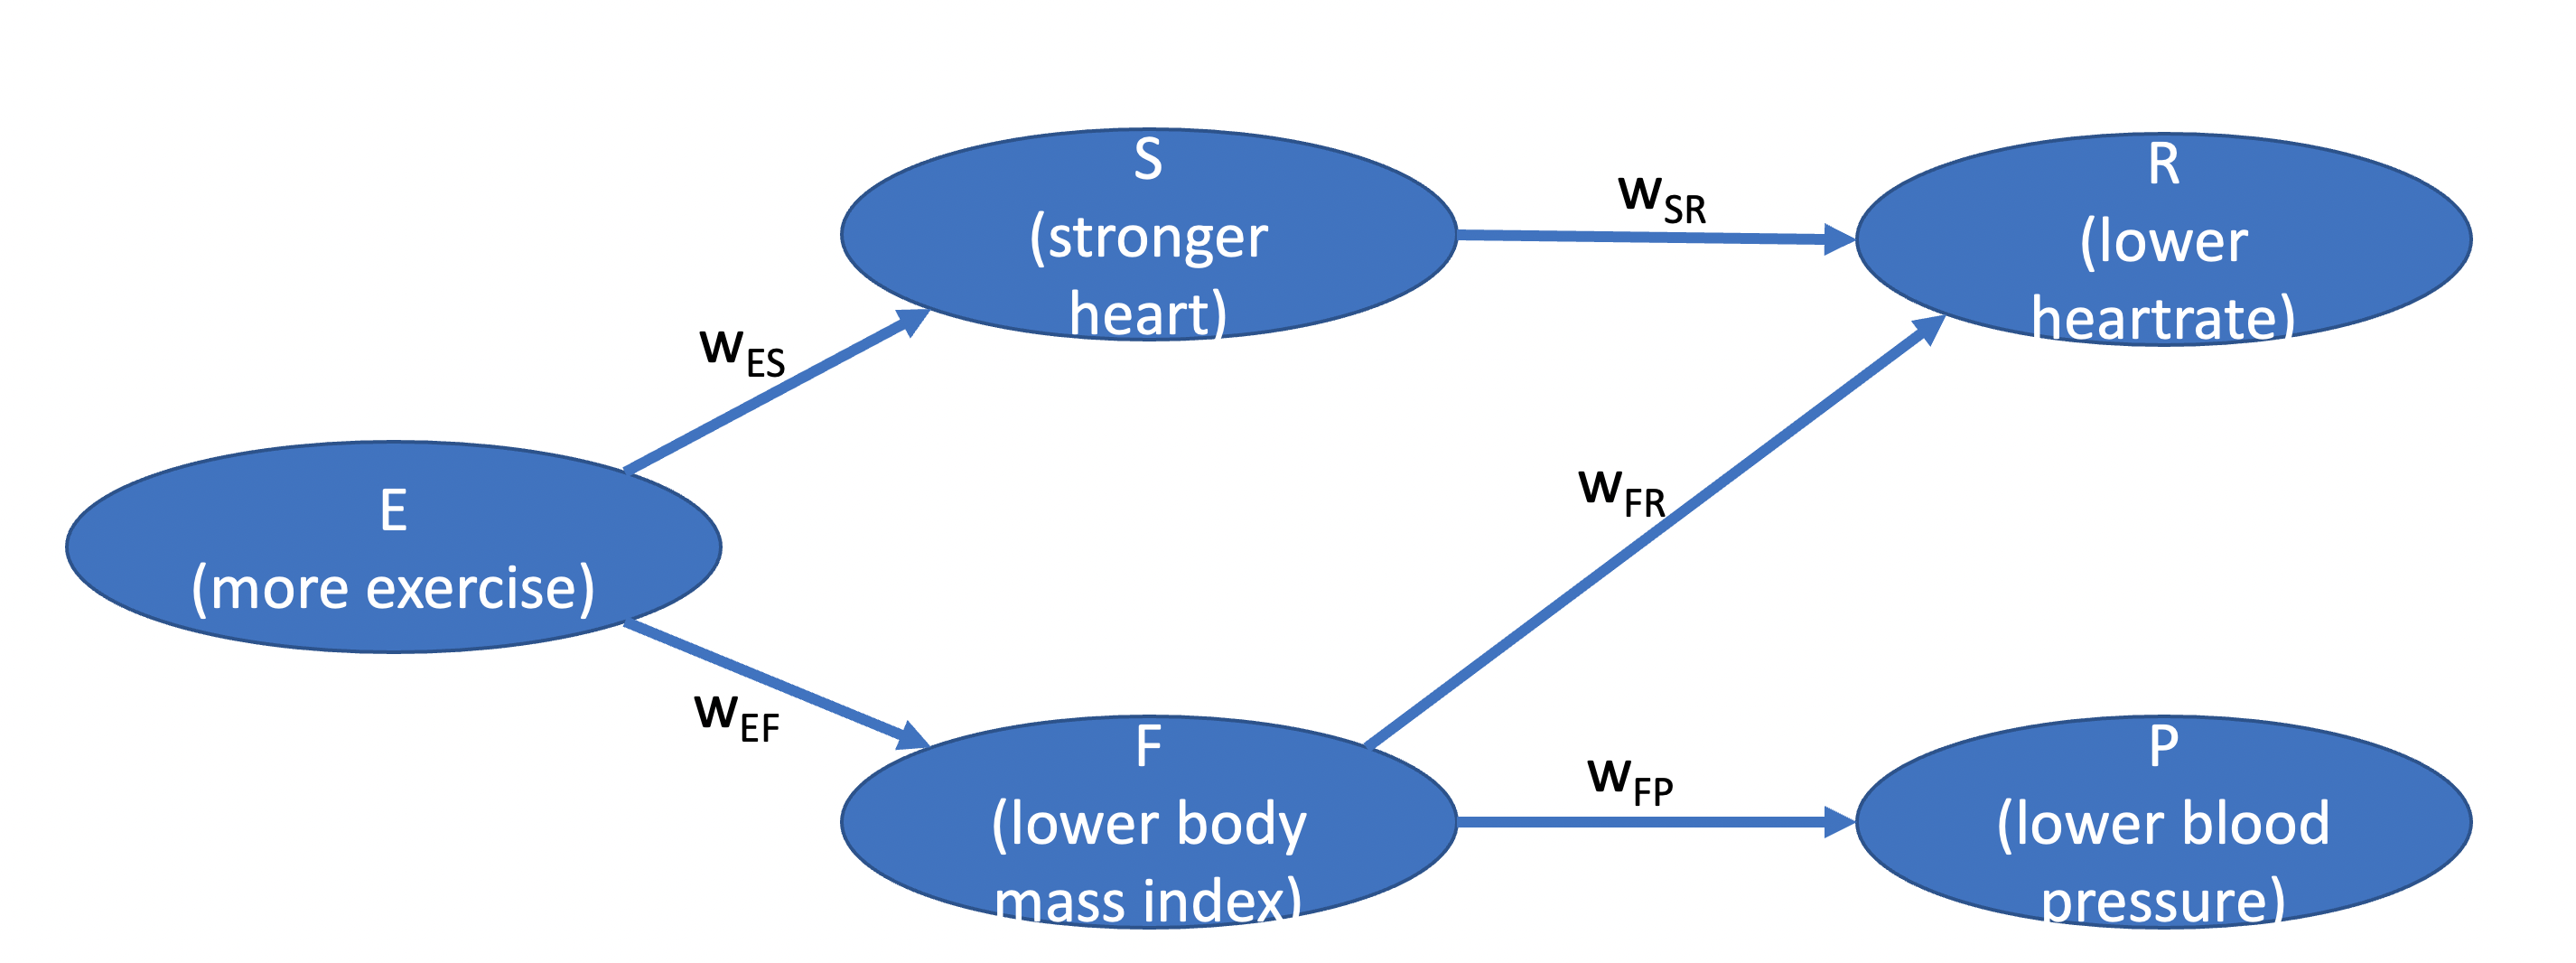
\includegraphics[width=12cm]{figures/scm_example_2.png}
\caption{\textbf{Example of a Structural Causal Model:} A Structural Causal model defines with variables are direct (noisy) functions of which other variables. In the figure above, S (stronger heart) is a direct function of E (exercise), hence there's a link between them. On the other hand, R (lower heart rate) is only influenced by E(exercise) through the mediation of S (stronger heart); hence there's no link between the two. }
\label{fig:scm_example}
\end{figure}

This graph simply summarizes what we know about which variables directly ``cause" which other variables (or which variables are direct functions of the others):
\begin{align}
    E &= U_{E} \\ 
    S &= f_{S}(E) + U_{S} \\
    F &= f_F(E) + U_{F} \\
    R &= f_R (S, F) + U_{R} \\
    P &= f_P (F) + U_{P}
\end{align}

In Figure \ref{fig:scm_example}, $E, S, F, R$ and $P$ are univariate random variables that represent exercise, heart strength, body mass index, heart rate and blood pressure, $U_E$, $U_S$, $U_F$, $U_R$ and $U_P$ are zero-centered (but not necessarily Gaussian) exogenous random variables and $f_S, f_F, f_R, f_P: \reals \mapsto \reals$ are functions that govern how causes impact their effects. The above set of variables and equations define a \textbf{Structural Causal Model} (SCM), also known as a \textbf{Structural Equation Model} -- a central abstraction in causal inference. 

Let's say the domain expert who gave us the above SCM also told us that the variables are linked to each other \textit{linearly} -- a very common assumption. This yields a linear SCM:

\begin{align}
    E &= U_{E} \\ 
    S &= w_{ES}E + U_{S} \\
    F &= w_{EF}E + U_{F} \\
    R &= w_{SR}S + w_{FR}F + U_{R} \\
    P &= w_{FP}F + U_{P}
\end{align}

Setting $\mV = [E, S, F, R, P]$ to be the concatenation of our random variables and $\mU = [U_E, U_S, U_F, U_R, U_P]$ the concatenation of the exogenous noise variables, we can succinctly express the SCM using matrix-vector notation: 
\begin{equation}
    \mV = \mW \mV + \mU \
\end{equation}

The matrix $\mW$ can be seen as the weighed adjacency matrix of the SCM: the nonzero entries $\mW_{ij}$ are equal to the weights connecting two nodes $i$ and $j$ connected with an edge. Note that $\mW$ is often quite sparse: $\mW_{ij} = 0$ if and only if there's no edge between two variables. 

What can we do with a given SCM topology? If we also know the weights, we can answer \textit{probabilistic and causal inference} type questions: given someones body-mass index and exercise habits, can we predict their expected blood pressure? If a person is given a medicine that strengthens heart muscle without directly affecting anything else, how does this affect ones heart rate? We can also attempt to \textit{learn} the coefficients in the linear SCM given a bunch of observations of the random variables: since the functional relationships between the variables is very clear, it's easy to set up a maximum likelihood objective and minimize it by optimizing over the SCM weights. 


\subsection{Structure Learning}
Above, the topology of the graph was given to us by a domain expert. Structure learning refer to the problem of learning the topology of SCM from data - a very difficult, yet very important learning problem. 

Let's formally state the structure learning problem following \citet{zheng2018dags} building on the formalism above. Let $\mX \in \reals^{n \times d}$ be a data matrix consisting of $n$ i.i.d. observations of the multivariable random variable $\mV$. Let $\mathbb{D}$ stand for the space of all DAGs on $d$ nodes. The purpose of structure learning is to learn a weighted adjacency matrix $\mW \in \reals^{d \times d}$ that not only models the dataset $\mX$ via the SCM equation $\mV = \mW\mV + \mU$, but also has the constraint that the edges defined by its nonzero entries describe a graph $G(V, E)$ that is a DAG (i.e. $G \in \dagspace)$). 

There are numerous ways of searching over the space of DAGs to find the most fitting one that describes the data. Until early 2010s, most approaches relied on discrete/combinatorial search algorithms (e.g \citet{heckerman1994combination}). \citet{zheng2018dags} take a different approach which uses a fully continuous optimization based algorithm to solve search over DAGs. This lecture is about the key technical contribution of this work, which is a novel loss function over adjacency matrices that quantify how "DAG-like" a graph is, with the level set corresponding to and only to DAGs. 

\textbf{The optimization problem: } We need three loss functions to set up our continuous optimization problem: (1) a loss function that quantifies how well the current $\mW$ estimate fits the data, (2) a regularization term to make sure the solution is well-behaved (sparse, for example), and (3) a constraint that guarantees that the $\mW$ found at the end of optimization represents a DAG. 

The choice of (1) and (2) are not central to this lecture, so we'll directly state what \citet{zheng2018dags} use:
\begin{align}
    F(W) = l(W, X) + r(W) = \frac{1}{2n} ||\mX - \mX \mW||_{F}^{2} + \lambda ||\mW||_1
\end{align}
The choice of $l$, besides making intuitive sense~\footnote{This loss has a maximum likelihood interpretation if one assumes that the exogenous noise terms are unit Gaussian.}, has solid theoretical backing: the minimizer of this loss "provably recovers a true DAG with high probability on finite samples and high-dimensions"~\citep{zheng2018dags}. The L1 loss on the adjacency matrix $\mW$ serves to enforce sparsity. It's not hard to show that the minimizer of L1 regularized least squares is sparse. The combination of these loss functions is analogous to LASSO regression~\citep{tibshirani1996regression}. 

The choice of (3) is the main contribution of \citep{zheng2018dags}, and deserves a whole section of its own. 

\section{Quantifying ``DAGness"}
We're in search of a function $h: \reals^{d \times d} \mapsto \reals$ that have the following properties:
\begin{enumerate}
    \item $h(\mW) = 0$ iff $\mW$ is acyclic. 
    \item High values of $h(\mW)$ implies that $G(\mW)$ has many cycles. Lower values imply not many cycles. 
    \item $h$ is smooth.
    \item $h$ and it's derivatives are easy to compute. 
\end{enumerate}

While it's relatively easy to satisfy (1) and (2) alone, satisfying all 4 criteria is challenging. 

\textbf{Candidate 1:} Pick $h(\mW)$ as the minimum L2 distance to an element of $\dagspace$:
\begin{align}
    h_{1}(\mW) = ||\mW - \proj_{\dagspace} \mW||_{F}
\end{align}
This loss function satisfies (1) and (2), but doesn't satisfy (3) and (4): it's derivatives are discontinuous and it's very difficult to differentiate through. (proof omitted)

Before considering $h(\mW)$ candidates, let's take a step back and consider what acyclicity really entails. For a graph to be a DAG, there should be no $k$-length cycles in it, for all values of $k$. If we could count the number of $k$-length cycles in a graph, then we could possibly use it to design a loss function to penalize $k$-length cycles. This insight leads to the following lemma:

\begin{lemma}
    Let $\mB \in \dagspace$ be the binary adjacency matrix of a directed graph G(V, E) of $d$ nodes. The number of paths starting at node $s$ and ending at node $t$, $p_{k}^{(st)}(\mB)$ is given by:
    \begin{equation}
        p_k^{(st)}(\mB) = \chi_{t}^T \mB^k \chi_{s} \label{eq:path_count}
    \end{equation}
    where $\chi_n$ is the indicator vector at node $n$. 
    \label{lemma:path_count}
\end{lemma}
\begin{proof}
    We'll use proof by induction. 
    The base case $k=1$ works, because $\chi_t^T \mB \chi_s = 1$ if $s$ and $t$ are neighbors (by the definition of an adjacency matrix) and $0$ otherwise. This is consistent with the definition $p_1^{(st)}$. 
    Now assume that the statement holds for $k-1$. This means that $(\mB^{k-1} \chi_s)_i = p_{k}^{(si)}(\mB)$. That is, $i$th coordinate of $\mB^{k-1}\chi_s$ contains the number of paths from $s$ to $i$. The total number of length $k$ paths that start from $s$ and leads to $t$ is equal to the sum of the number of all $k-1$ length paths that start at $s$ and lead to a neighbor of $t$. Combining this with the definition of an adjacency matrix, we conclude the proof.
    \begin{align}
        p_{k}^{(st)} &= \sum_{u: (u, t) \in E} p_{k-1}^{(si)}
        = \sum_{i=1}^{d}\mB_{ti} p_{k-1}^{(si)} 
        = \sum_{i=1}^{d} \mB_{ti} (\mB^{k-1}\chi_s)_i 
        = \chi_t^T B B^{k-1} \chi_s 
        = \chi_t^T B^k \chi_s
    \end{align}
\end{proof}
Now that we can count the number of paths with known start and end nodes, we can count the total number of $k$-length cycles in a graph. 
\begin{lemma}
    Let $\mB \in \dagspace$ be the binary adjacency matrix of a directed graph G(V, E) of $d$ nodes. The total number of $k$-length cycles in $G$, $c_k(\mB)$, is given by:
    \begin{equation}
        c_k (\mB) = \Tr \mB^k
    \end{equation}
    \label{lemma:num_k_cycles}
\end{lemma}
\begin{proof}
    The total number of length $k$ paths starting and ending on node $s$ is given by $p_k^{(ss)} (\mB) = \chi_s^T \mB^k \chi_s$ (by Lemma \ref{lemma:path_count}). Counting length $k$ cycles starting on all nodes, we get:
    \begin{align}
        c_k(\mB) = \sum_{i=1}^{d} p_{k}^{(ii)} = \sum_{i=1}^{d} (\mB^k)_{ii} = \Tr \mB^k
    \end{align}
\end{proof}

We're now ready to state a new candidate loss function. 

\textbf{Candidate 2:} Pick $h(\mW)$ as follows:
\begin{align}
    h_2(\mW) = \Tr (\mI - \mW)^{-1} - d
\end{align}

While the inverse might look counter-intuitive, things become conceptually cleaner when one considers the (matrix version of the) identity $\frac{1}{1-x} = 1 + x + x^2 + x^3 \dots$ Now, let's justify this loss function more formally. 
\begin{lemma}
     Let $\mB \in \dagspace$ be the binary adjacency matrix of a directed graph G(V, E) of $d$ nodes. Further assume that $r(\mB) < 1$ where $r(\mB)$ is the largest singular value of $\mB$. Then $\mB$ is a DAG if and only if 
     \begin{align}
         \Tr (\mI - \mB)^{-1} = d
     \end{align}
\end{lemma}
\begin{proof}
    $\mB$ is a DAG if and only if it doesn't contain any cycles. By Lemma \ref{lemma:num_k_cycles} this is equivalent to saying $\Tr \mB^k = 0$ for any $k \geq 1$. By the Neumann sum identity, we can write:
    \begin{align}
        \Tr (\mI - \mB)^{-1} = \Tr \sum_{i=0}^{\infty}\mB^k = \Tr \mI + \sum_{i=1}^{\infty}\Tr \underbrace{\mB^k}_{\text{=0 for all k larger than 1}} = d
    \end{align}
\end{proof}

This loss function (or the version where infinity is replaced with $d$ to the same effect) is quite promising, while having fatal flaws. First, we need to ensure $r(\mW) < 1$ throughout training, which prevents learning to discover SCM formulas that don't satisfy these properties. Moreover, values of $\Tr \mB^k$ can get extremely large if the graph is large enough, exceeding machine precision and preventing reliable gradients from being calculated. 

Luckily, there exists a loss function that solves both of these issues. 

\textbf{Candidate 3: } Pick $h$ as follows:
\begin{align}
    h(\mW) = \Tr \exp (\mW \circ  \mW) - d
\end{align}
where $\circ$ stand for Hadamard product and $\exp$ stand for matrix exponential. 
Intuitively, this works because just like the inverse operation in Candidate 2, Candidate 3 also defines an infinite sum over the k-length cycles in the graph, but this time weighed by $\frac{1}{k!}$. Let's now see this more concretely. 

\begin{lemma}
     Let $\mB \in \dagspace$ be the binary adjacency matrix of a directed graph G(V, E) of $d$ nodes. $\mB$ is a DAG iff 
     \begin{align}
         \Tr \exp \mB = d
     \end{align}
\end{lemma}
\begin{proof}
    Following the definition of the matrix exponential, we get:
    \begin{align}
        \Tr \exp \mB &= \Tr \sum_{i=0}^{\infty} \frac{1}{k!} \mB^k
        = \Tr \mI + \sum_{i=1}^{\infty} \frac{1}{k!} \mB^k  = d + \sum_{i=1}^{\infty} \frac{1}{k!} \mB^k \label{eq:exp_cycle}
    \end{align}
    By Lemma \ref{lemma:num_k_cycles}, we have that the right hand of Equation \ref{lemma:num_k_cycles} is $0$ (i.e. $\Tr \mB^k=0$ for all $k \geq 1$) iff $\mB$ is a DAG, completing the proof. 
\end{proof}

As stated above, moving from the inverse operation to matrix exponential merely adds a $\frac{1}{k!}$ scaling to each term in the infinite sum. this serves two crucial purposes: 1) Now, we don't have any constraint on the spectral radius! This loss function works on any matrix. 2) Larger length step counts are normalized by a factor that grows exponentially with $k$. Moreover, it's now smooth and differentiable!
\begin{lemma}
    The gradient of the (candidate 3) loss function $h(\mB)$ is given by:
    \begin{align}
        \grad h(\mW) = 2(\exp \mW \circ \mW) \circ \mW
    \end{align}
\end{lemma}
The proof for this is trivial and hence omitted. 

Candidate 3 satisfies all of the desiderata, hence can be used to fully define the NOTEARS optimization problem:

\begin{align}
    &\min_{\mW \in \reals^{d \times d}} \frac{1}{2n} ||\mX - \mX \mW||_{F}^{2} + \lambda ||\mW||_1 \\
    &\text{subject to} \quad h(\mW) = \Tr \exp (\mW \circ  \mW) - d = 0
\end{align}

While well defined, this objective is unfortunately non-convex, since the loss function $h$ is nonconvex. (Nonconvexity is inevitable, as the space of DAGs is non-convex) We'll now discuss how the augmented Lagrangian machinery can be used to solve this constrained minimization problem to great empirical success. 


% \begin{itemize}
%     \item Give motivating example. 
%     \begin{itemize}
%         \item Define PGMs. Give an example. 
%         \item Define what one can do with a given PGM (i.e. do inference or learn parametric distributions).
%         \item Tell that structure learning is the significantly more difficult problem of inferring the graph structure from data alone. Give an example. (protein and phospholipids in immune cells dataset). 
%         \item Why is this an interesting problem?
%         \begin{itemize}
%             \item Useful for scientific discovery
%             \item Useful for causal discovery
%         \end{itemize}
        
%     \end{itemize}
%     \item Introduce notation. 
%     \begin{itemize}
%         \item X: data matrix. 
%         \item D: (discrete) space of DAGs.
%         \item Assumption: each variable is a noisy linear combination of the others. 
%         \item W: Defines the adjacency matrix. When an entry is not zero, it quantifies the connection between edges. 
%         \item Describe the induced SEM. 
%         \begin{itemize}
%             \item Add 1) Equations, 2) Graphical model, 3) the adjacency matrix W. 
%         \end{itemize}
%         \item Linear SEMs can model any generalized linear model. 
%     \end{itemize}
%     \item Emphasize that this graph is directed. Hence, the adjacency matrix is not symmetric. 
%     \item Introduce linear vs. non-linear SEMs. 
%     \item Introduce loss function. 
%     \begin{itemize}
%         \item Desirable properties of least squares
%         \item Sparsity inducing L1 loss. 
%     \end{itemize}
% \end{itemize}   


% \section{Continuous Optimization Formulation}
% \begin{itemize}
%     \item Desiderata. 
%     \item Counting length-k walks. 
%     \item Introduce infinite series loss.
%     \begin{itemize}
%         \item Make connection to random walks
%         \item Mention it requires the radius to be less than 1. 
%     \end{itemize}
%     \item Introduce the exponential loss. 
% \end{itemize}



\section{Optimizing the NOTEARS Objective}
As mentioned in the previous section, the optimization problem is non-convex since the constraint $h(\mW)=0$ defines a non-convex set.
This implies that having the gradient of the Lagrangian equal to zero at some point $\mW$ (i.e., a \emph{stationary point}) is not a sufficient condition for optimality.
Nonetheless, experiments show that said stationary points are close enough to the true optimum for the applications considered.

The authors apply the augmented Lagrangian method to solve the optimization problem, which adds a quadratic penalty $\frac{\rho}{2}|h(\mW)|^2$ to the objective function resulting in

\begin{align}
    &\min_{\mW \in \reals^{d \times d}} \frac{1}{2n} ||\mX - \mX \mW||_{F}^{2} + \lambda ||\mW||_1 + \alpha h(\mW) + \frac{\rho}{2}|h(\mW)|^2 \\
    &\text{subject to} \quad h(\mW) = \Tr \exp (\mW \circ  \mW) - d = 0.
\end{align}
Note that $h(\mW)=0$ whenever $\mW$ is a solution. Hence, adding the quadratic penalty will not change the solution set with respect to the original optimization problem.
Intuitively, as $\rho$ increases, any convex solver will increasingly favor solution where $|h(\mW)|$ is closer to zero.
A full treatment of this method is beyond the scope of the write-up.

Converting the constrained optimization problem above into a non-constrained one yields the following objective
\begin{align}
    \max_{\alpha \in \reals} \min_{\mW \in \reals^{d \times d}} F(\mW) + \frac{\rho}{2}|h(\mW)|^2 + \alpha h(\mW),
\end{align}
where $F(\mW) = \frac{1}{2n} ||\mX - \mX \mW||_{F}^{2} + \lambda ||\mW||_1$.
As previously mentioned, it will suffice to find a local minimizer $\mW^\star_\alpha$ for the inner loop at some value of $\alpha$. There are a multitude of different black-box solvers that can efficiently find globally and locally optimal solutions for convex and non-convex problems, respectively. The development of such programs are completely orthogonal to the specific domain of the optimization problem and is out of the scope for this write-up and hence shall not be discussed. The outer loop can be optimized via gradient descent methods by noting that
\begin{align}
    \nabla_\alpha \left( F(\mW^\star_\alpha) + \frac{\rho}{2}|h(\mW^\star_\alpha)|^2 + \alpha h(\mW^\star_\alpha) \right) = h(\mW^\star_\alpha).
\end{align}

Finally, because the chosen convex solvers will not necessarily output an estimate $\tilde{\mW}$ with some entries equal to $0$ (i.e., indicating an absence of an edge in the DAG), the method requires specifying a threshold value $\omega \geq 0$ where all entries in $\tilde{\mW}$ smaller than $\omega$ are set to zero. Note that the thresholding step has non-trivial consequences: a hard-thresholding step with an appropriately chosen value reduces the number of false discoveries \citep{zhou2009thresholding}. 

\section{Results and Discussion}
The authors provide comparisons with existing methods on both toy examples (i.e., synthetic data) and real-world datasets.

For each experiment a graph is sampled from either the Erdős–Rényi (ER) or scale-free (SF) families of random graphs along with a ground truth weight matrix $\mW$. Then, $\mV = \mX\mV + \mU$ is sampled using either a Normal, Exponential or Gumbel distribution for $\mU$ to generate datasets $\mX \in \reals^{n \times d}$ for multiple values of $n$ and $d$. For each experiment, the following 3 analyses are presented.

\paragraph{Parameter estimation:} In Figures 1. and 2.~\footnote{These figures are screenshots from the original paper. Hence, the captions belong to the authors. } a visual comparison between the estimated and ground truth weight matrices, $\tilde{\mW}$ and $\mW^\star$, is provided for different threshold values $\omega$.
The results indicate that, at least for these simple experiments and through visual inspection, the method can recover the underlying ground truth.


\begin{figure}[h]
\center
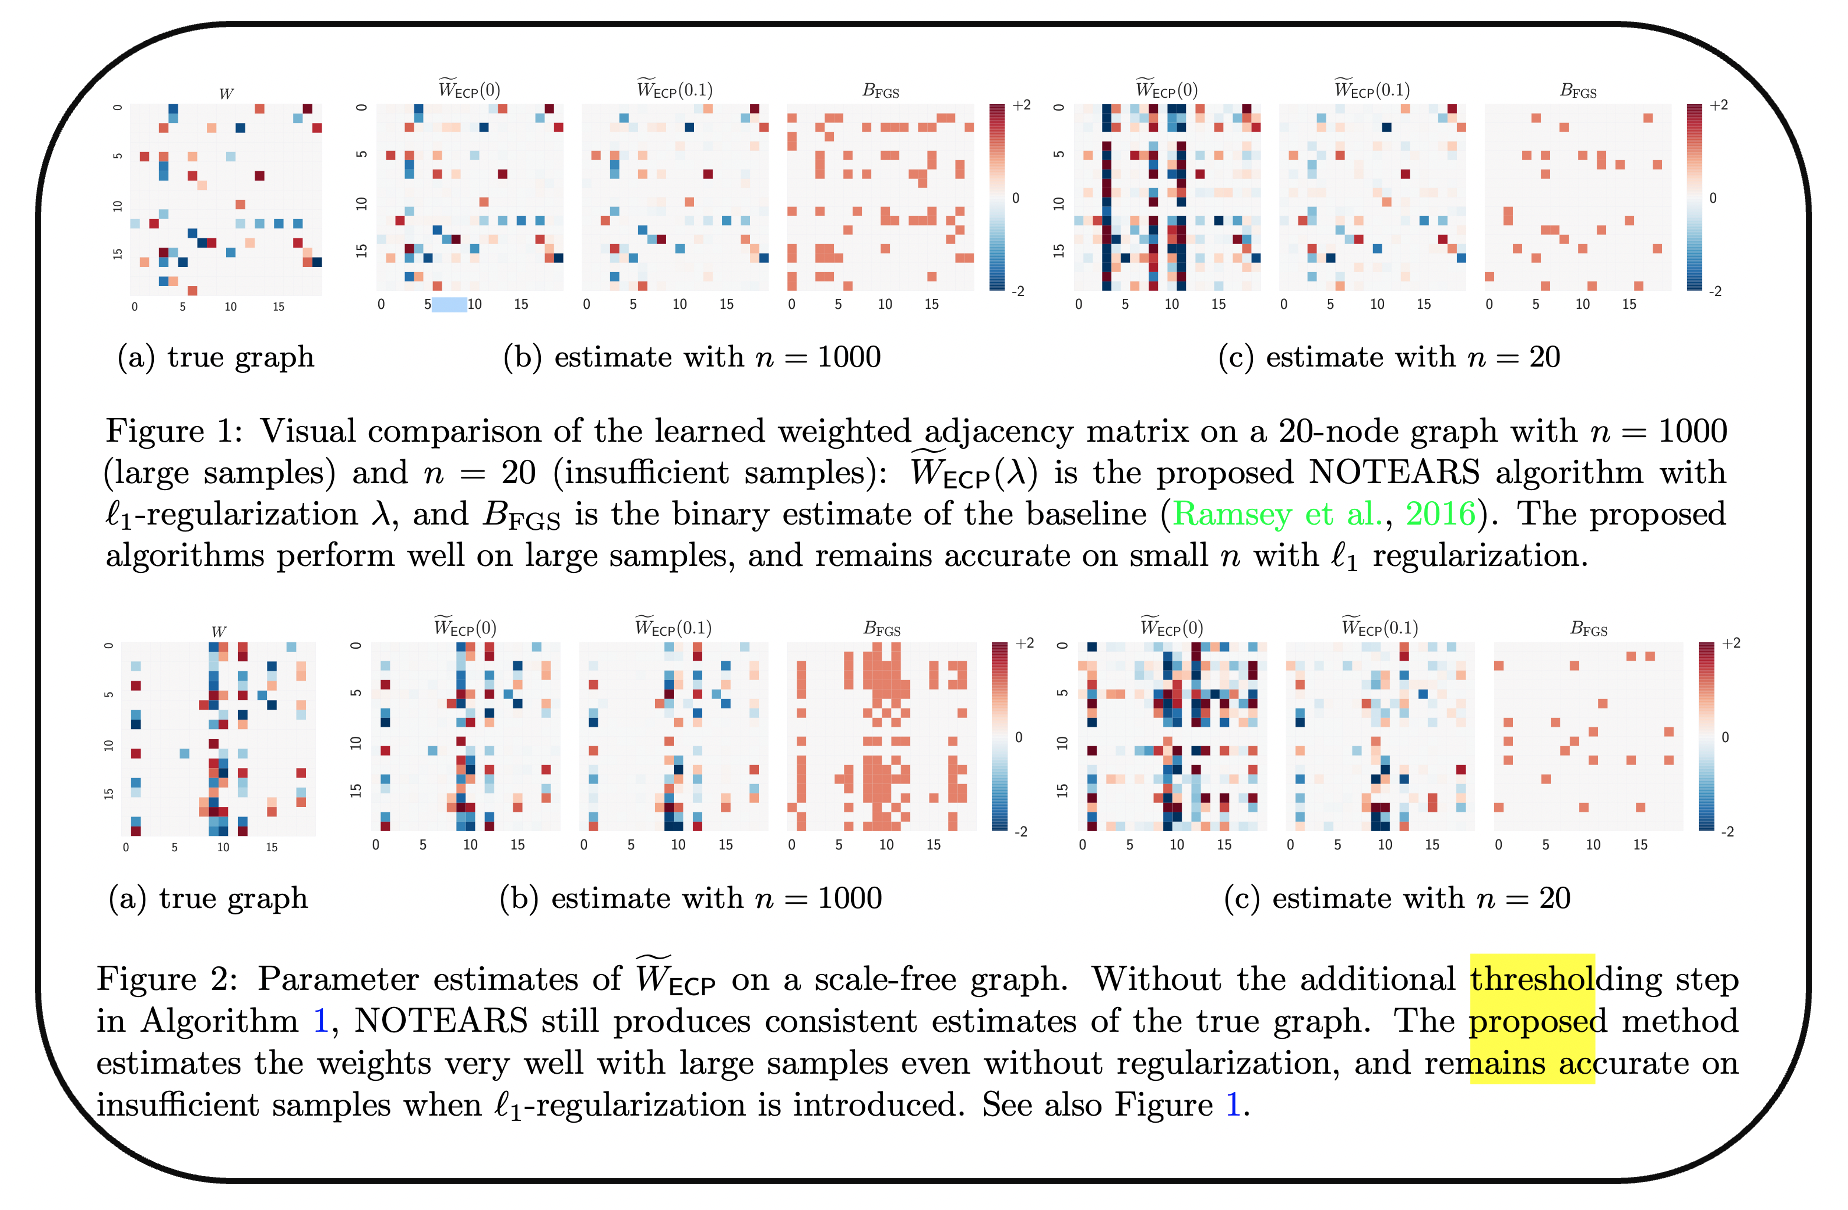
\includegraphics[width=16cm]{figures/fig1_and_2.png}
% \caption{\textbf{Example of a Structural Causal Model:} A Structural Causal model defines with variables are direct (noisy) functions of which other variables. In the figure above, S (stronger heart) is a direct function of E (exercise), hence there's a link between them. On the other hand, R (lower heart rate) is only influenced by E(exercise) through the mediation of S (stronger heart); hence there's no link between the two. }
\label{fig:figs_1_2}
\end{figure}

\paragraph{Structure Learning:} A common way to compare 2 graphs is through the \emph{Hamming Distance}, which measures the minimal number of edits (e.g., addition and removal of edges)  required to transform one graph to another. The Hamming Distance is compared for varying values of $n, d$, distributions for $\mU$, and random graph families. NOTEARS consistently outperforms other methods for large values of $n$ and $d$, but under-performs for small values of $n$ (i.e., when there is little data) -- see Figure 3. 

\begin{figure}[h]
\center
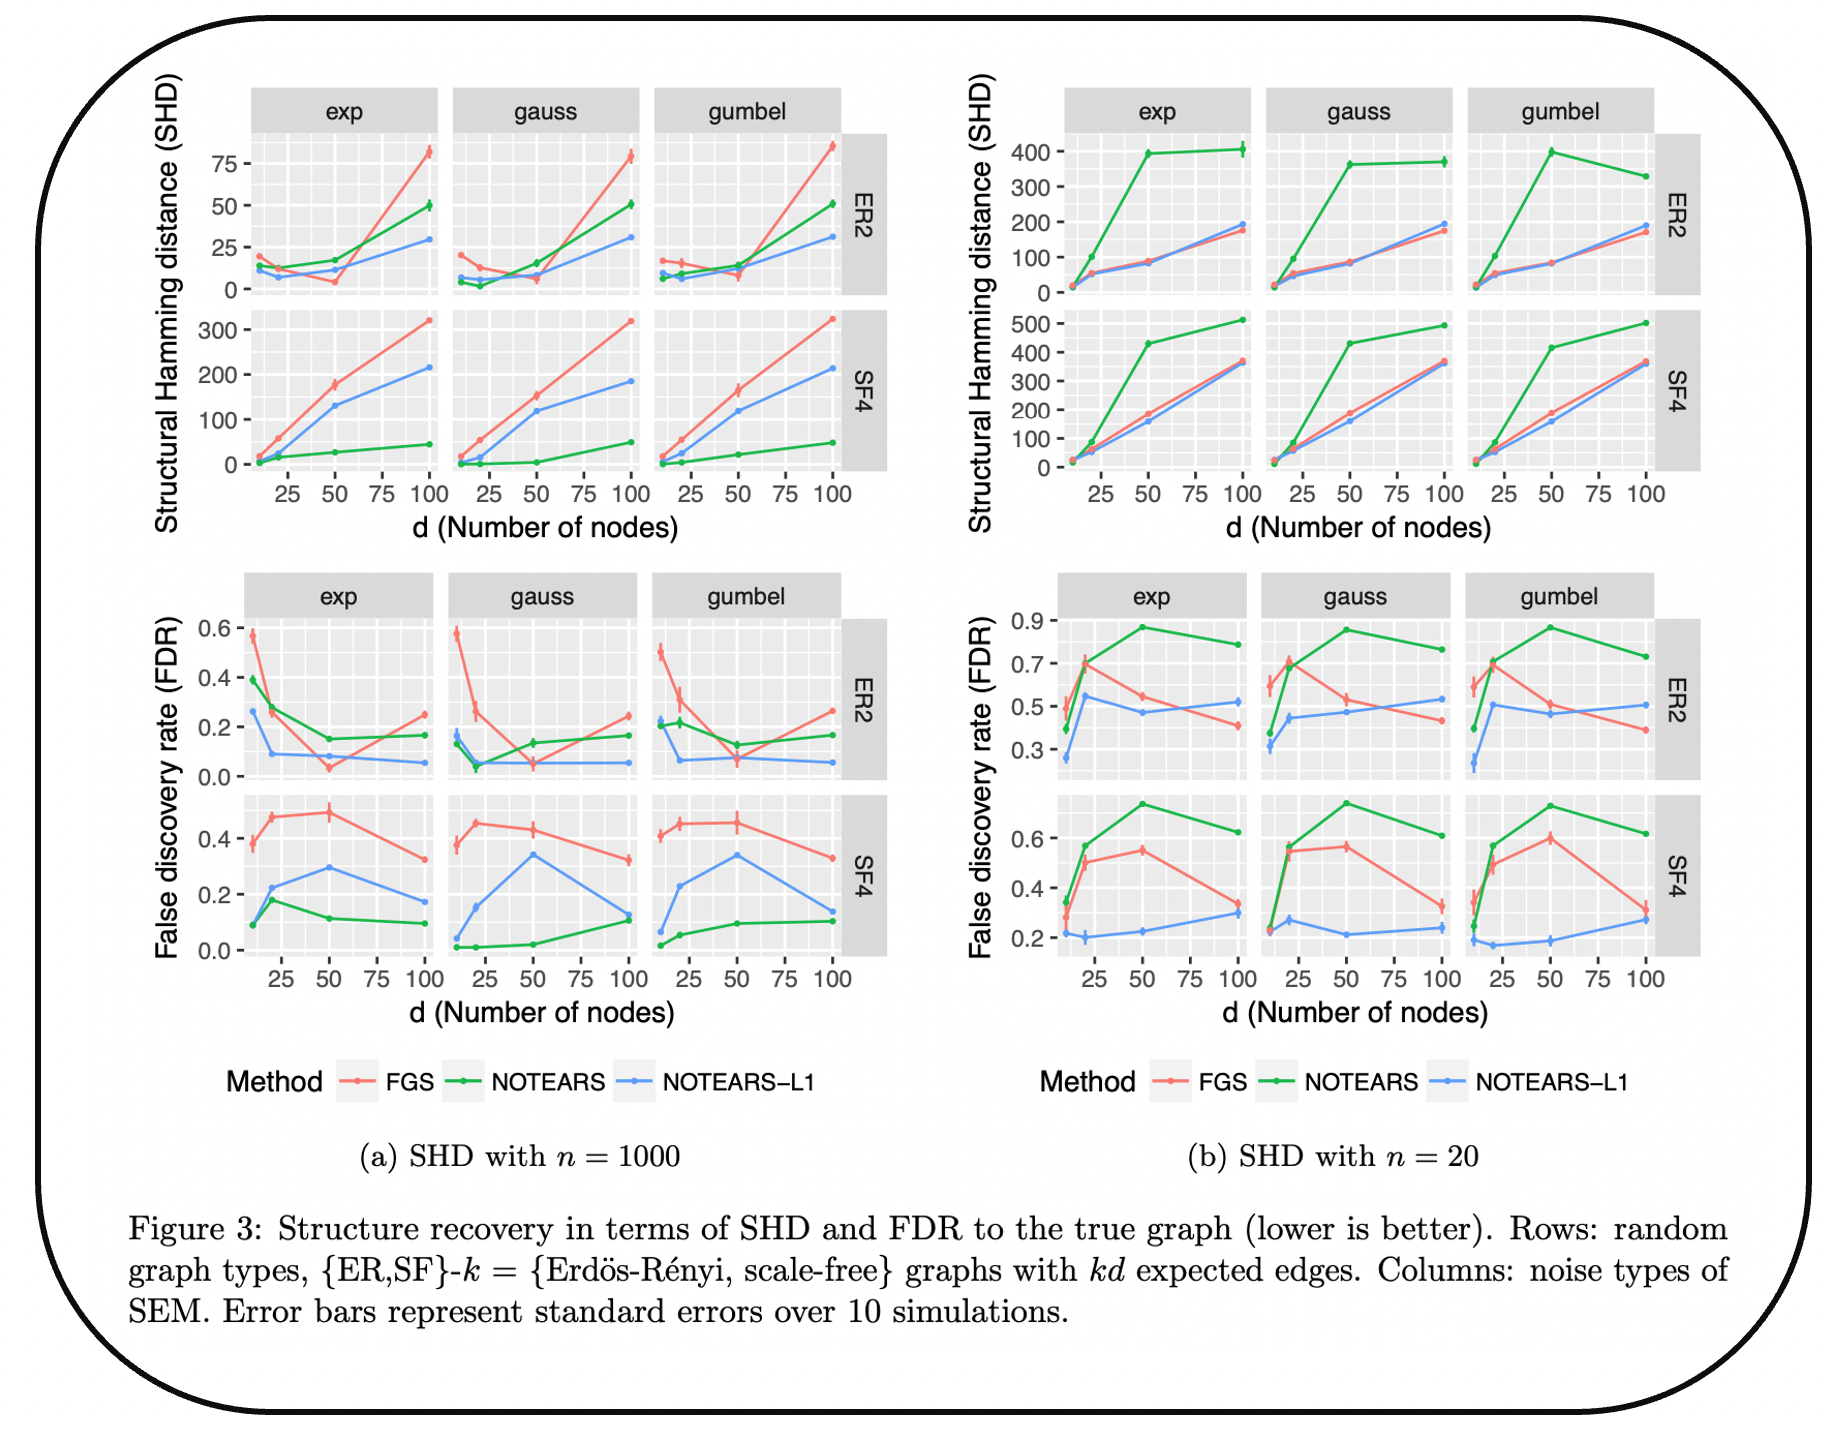
\includegraphics[width=16cm]{figures/fig3.png}
% \caption{\textbf{Example of a Structural Causal Model:} A Structural Causal model defines with variables are direct (noisy) functions of which other variables. In the figure above, S (stronger heart) is a direct function of E (exercise), hence there's a link between them. On the other hand, R (lower heart rate) is only influenced by E(exercise) through the mediation of S (stronger heart); hence there's no link between the two. }
\label{fig:fig3}
\end{figure}


\paragraph{Comparison to exact global minimizer:} For small DAGs it is possible to find the global optimum of the NOTEARS objective in feasible time using out-of-the-box solvers.
In this setting the dimensionality is fixed to $d=10$ and $n$ is varied from $20$ to $1000$.
The error of NOTEARS estimate $\tilde{\mW}$ with respect to the global objective $\mW^\star$ is measured as $||\tilde{\mW} - \mW^\star||$, which is shown to be small (compared to the norm of $\mW^\star$).
This indicates that the non-convexity of the NOTEARS objective does not significantly hinder the employment of convex solvers, at least for low dimensionality -- Table 1. 

\begin{figure}[ht!]
\center
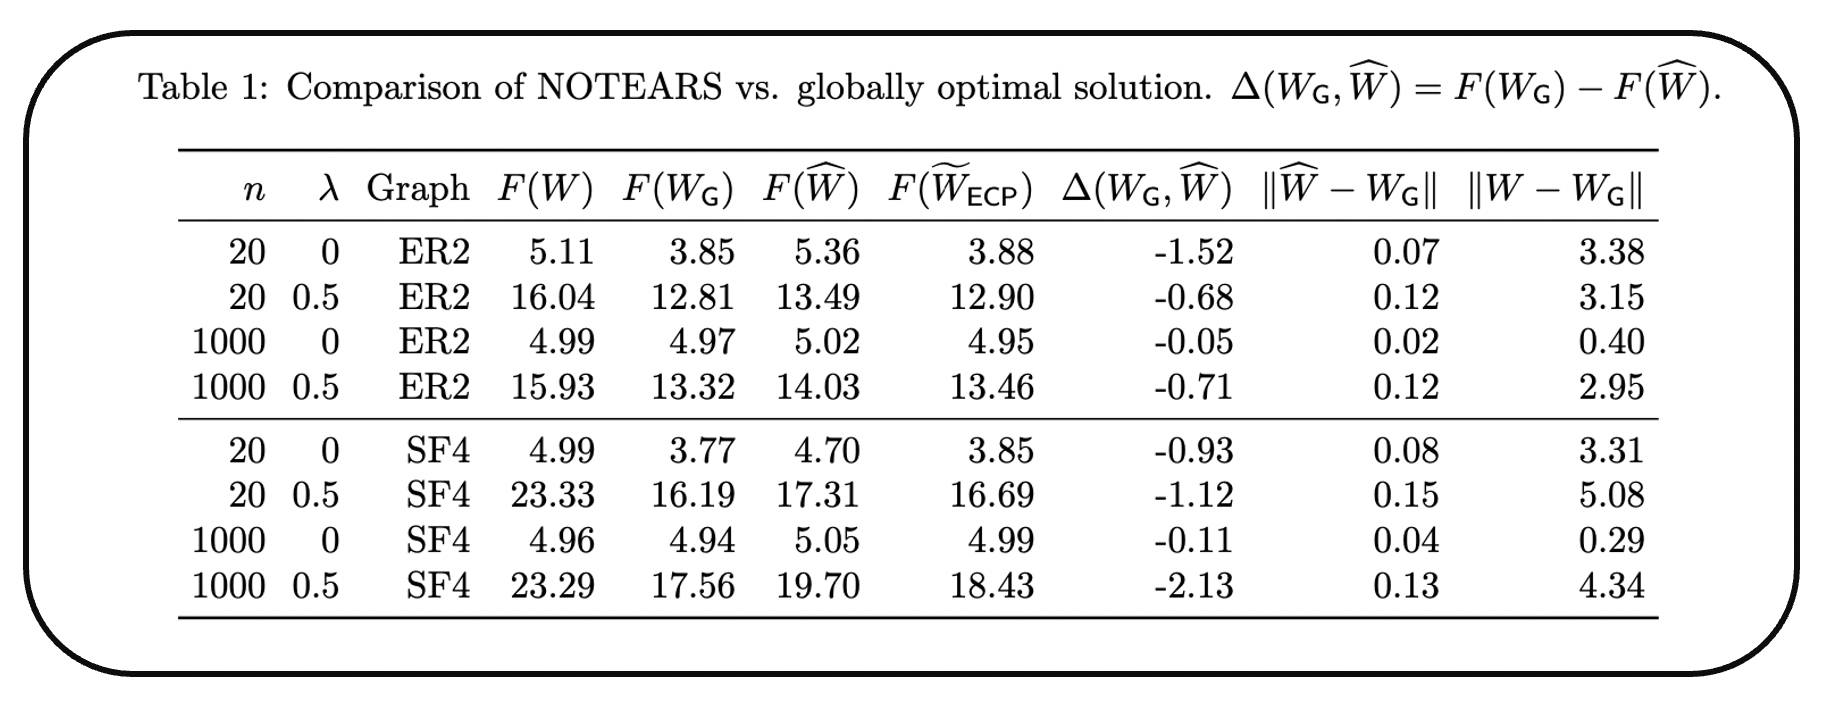
\includegraphics[width=16cm]{figures/tab1.png}
% \caption{\textbf{Example of a Structural Causal Model:} A Structural Causal model defines with variables are direct (noisy) functions of which other variables. In the figure above, S (stronger heart) is a direct function of E (exercise), hence there's a link between them. On the other hand, R (lower heart rate) is only influenced by E(exercise) through the mediation of S (stronger heart); hence there's no link between the two. }
\label{fig:figs_1_2}
\end{figure}

\bibliography{references}
\bibliographystyle{apalike} 

\clearpage
\appendix

\end{document}
